\section{Algorithm Results}
The results of the algorithms accord to the methods above are as follows.

\subsection{AdaBoost}
\begin{figure}[H]
    \centering
    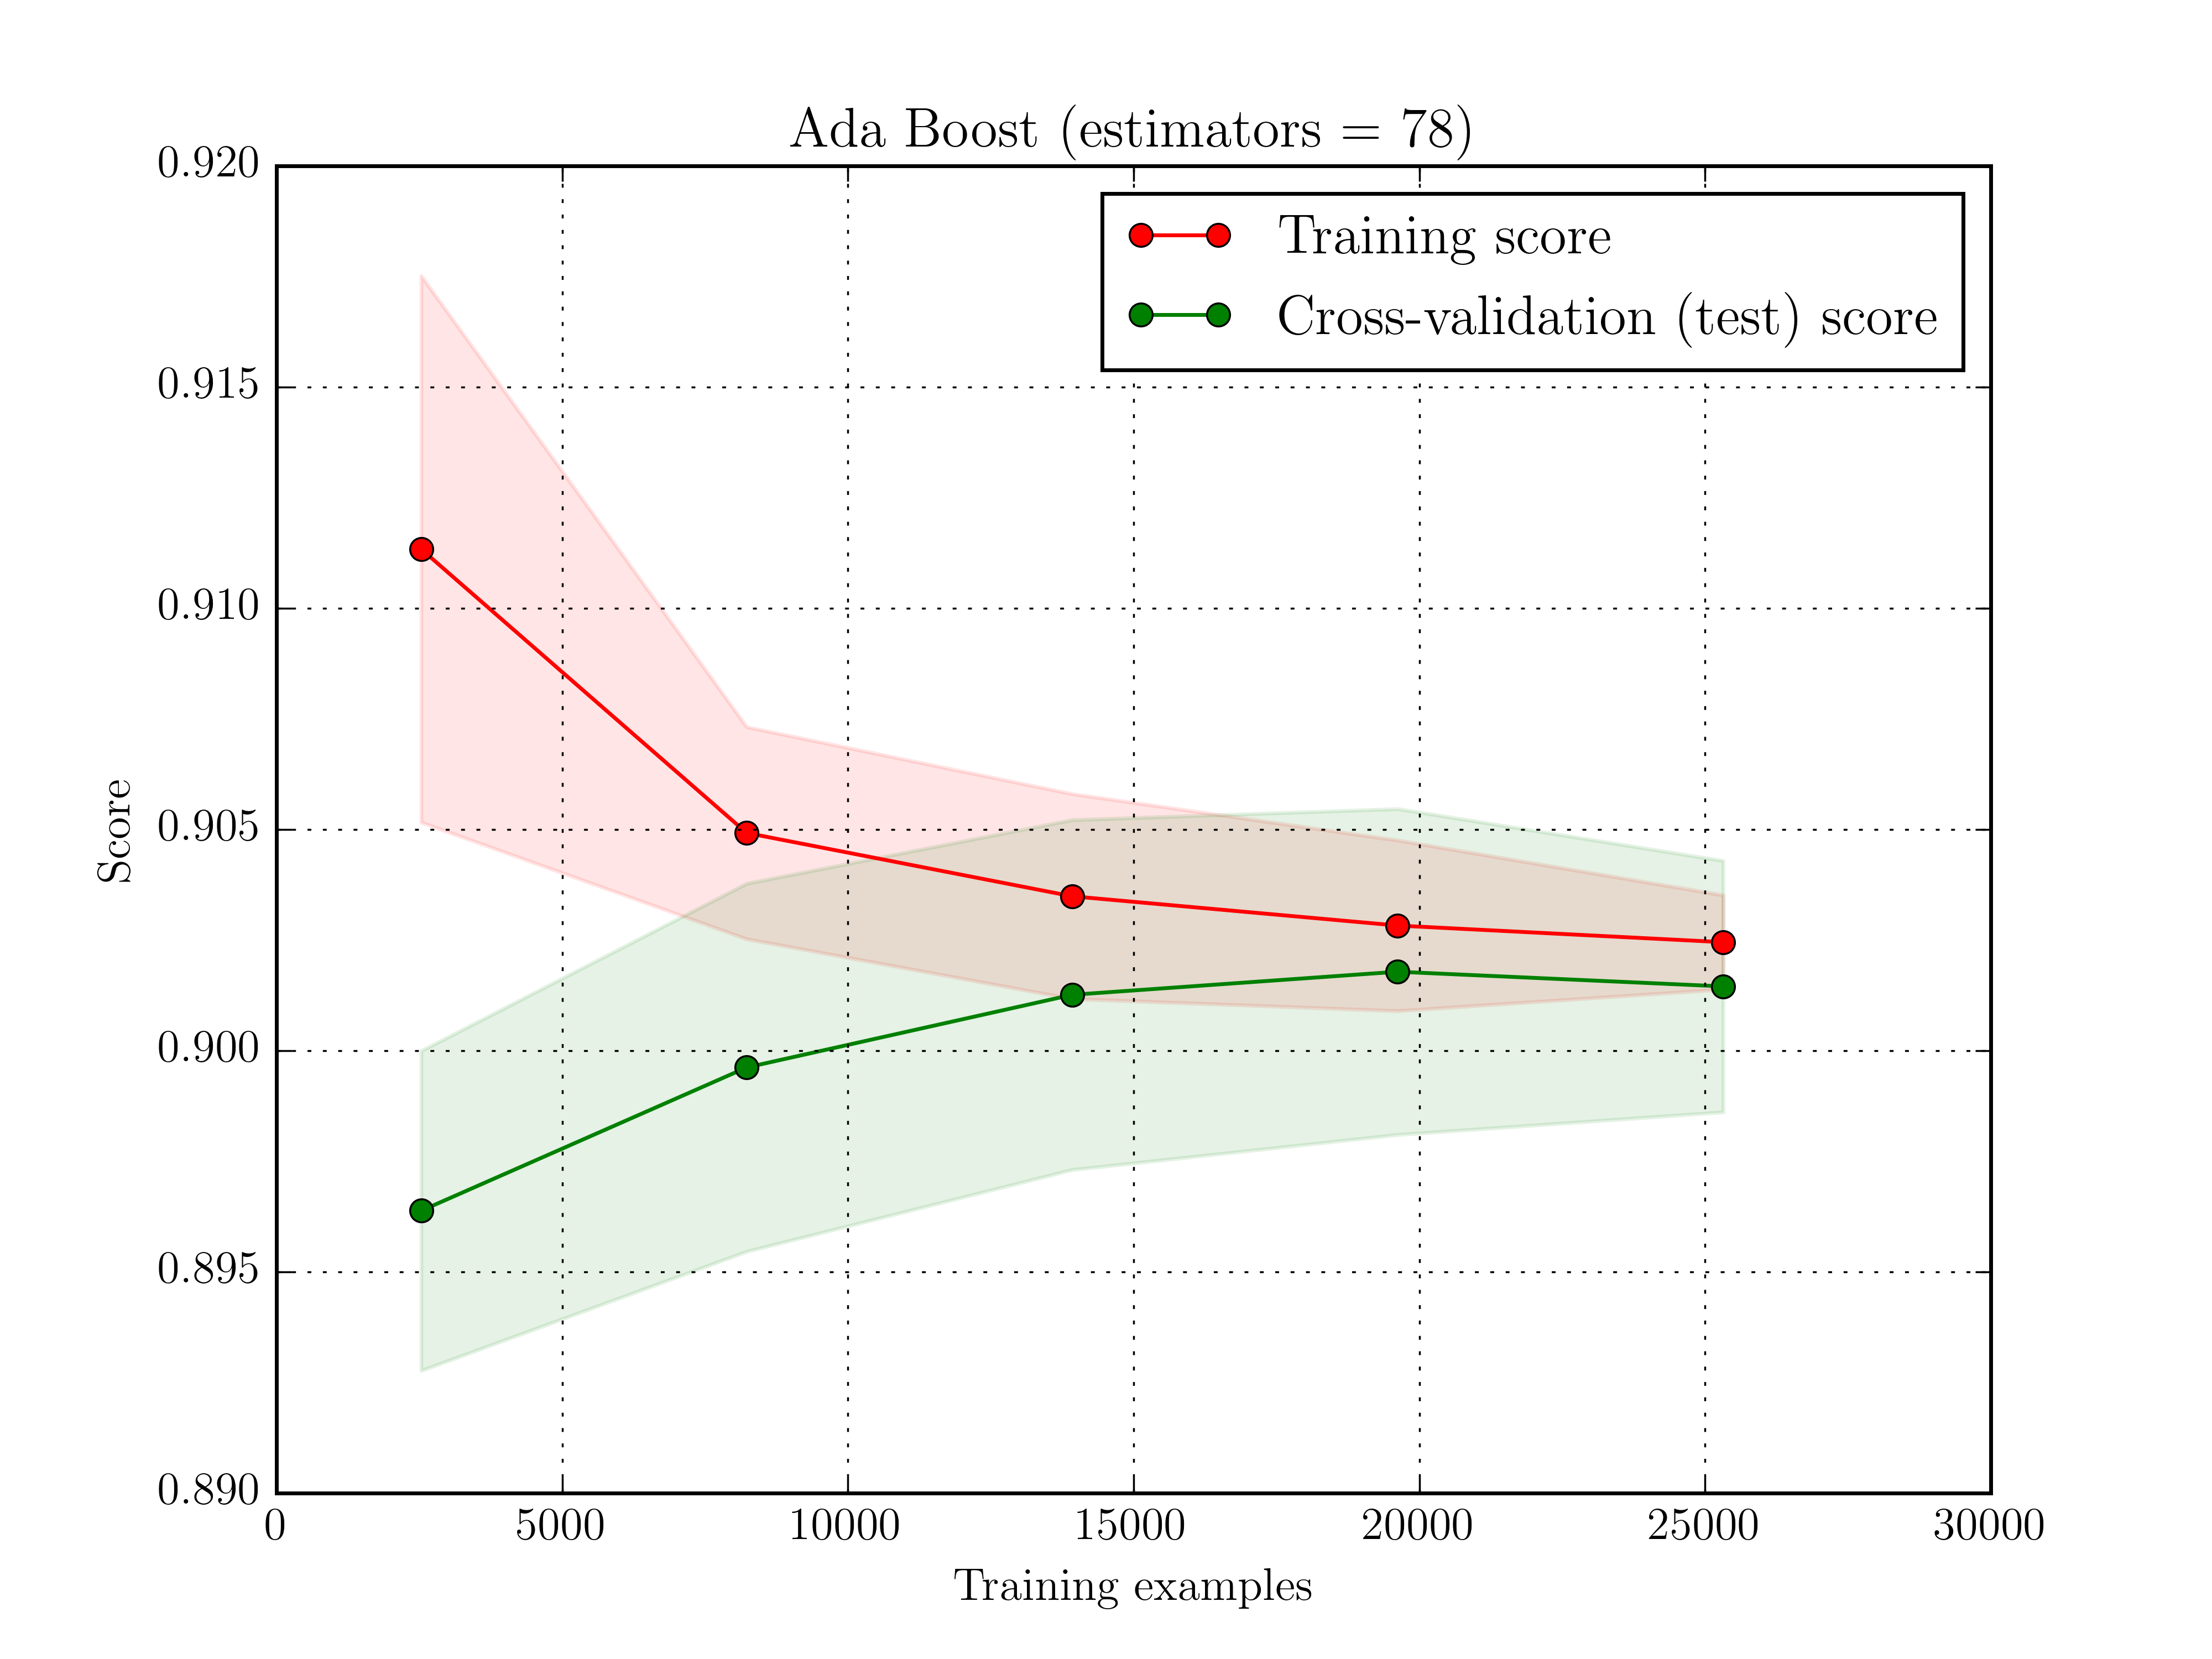
\includegraphics[width=.7\textwidth]{bank/boost.png}
    \caption{AdaBoost with decision tree estimators on bank marketing data set. Runtime: 14 minutes}
\end{figure}

The following is a table for accuracy values for other estimators retrieved from the grid search algorithm.
The most accurate number of estimators (the one that is graphed) is shown in bold.
\begin{center}
    \begin{tabular}{l|| c | c | c | c | c | c | c | c | c | c}
        \# est. = & 18    & 26    & 37    & 54    & \textbf{78}    & 112   & 162   & 233   & 335   & 483\\
         \hline
         mean & 0.897 & 0.898 & 0.900 & 0.900 & \textbf{0.903} & 0.900 & 0.902 & 0.902 & 0.902 & 0.902\\
         std  & 0.001 & 0.002 & 0.003 & 0.003 & \textbf{0.002} & 0.004 & 0.001 & 0.005 & 0.003 & 0.003
    \end{tabular}
\end{center}

\begin{figure}[H]
    \centering
    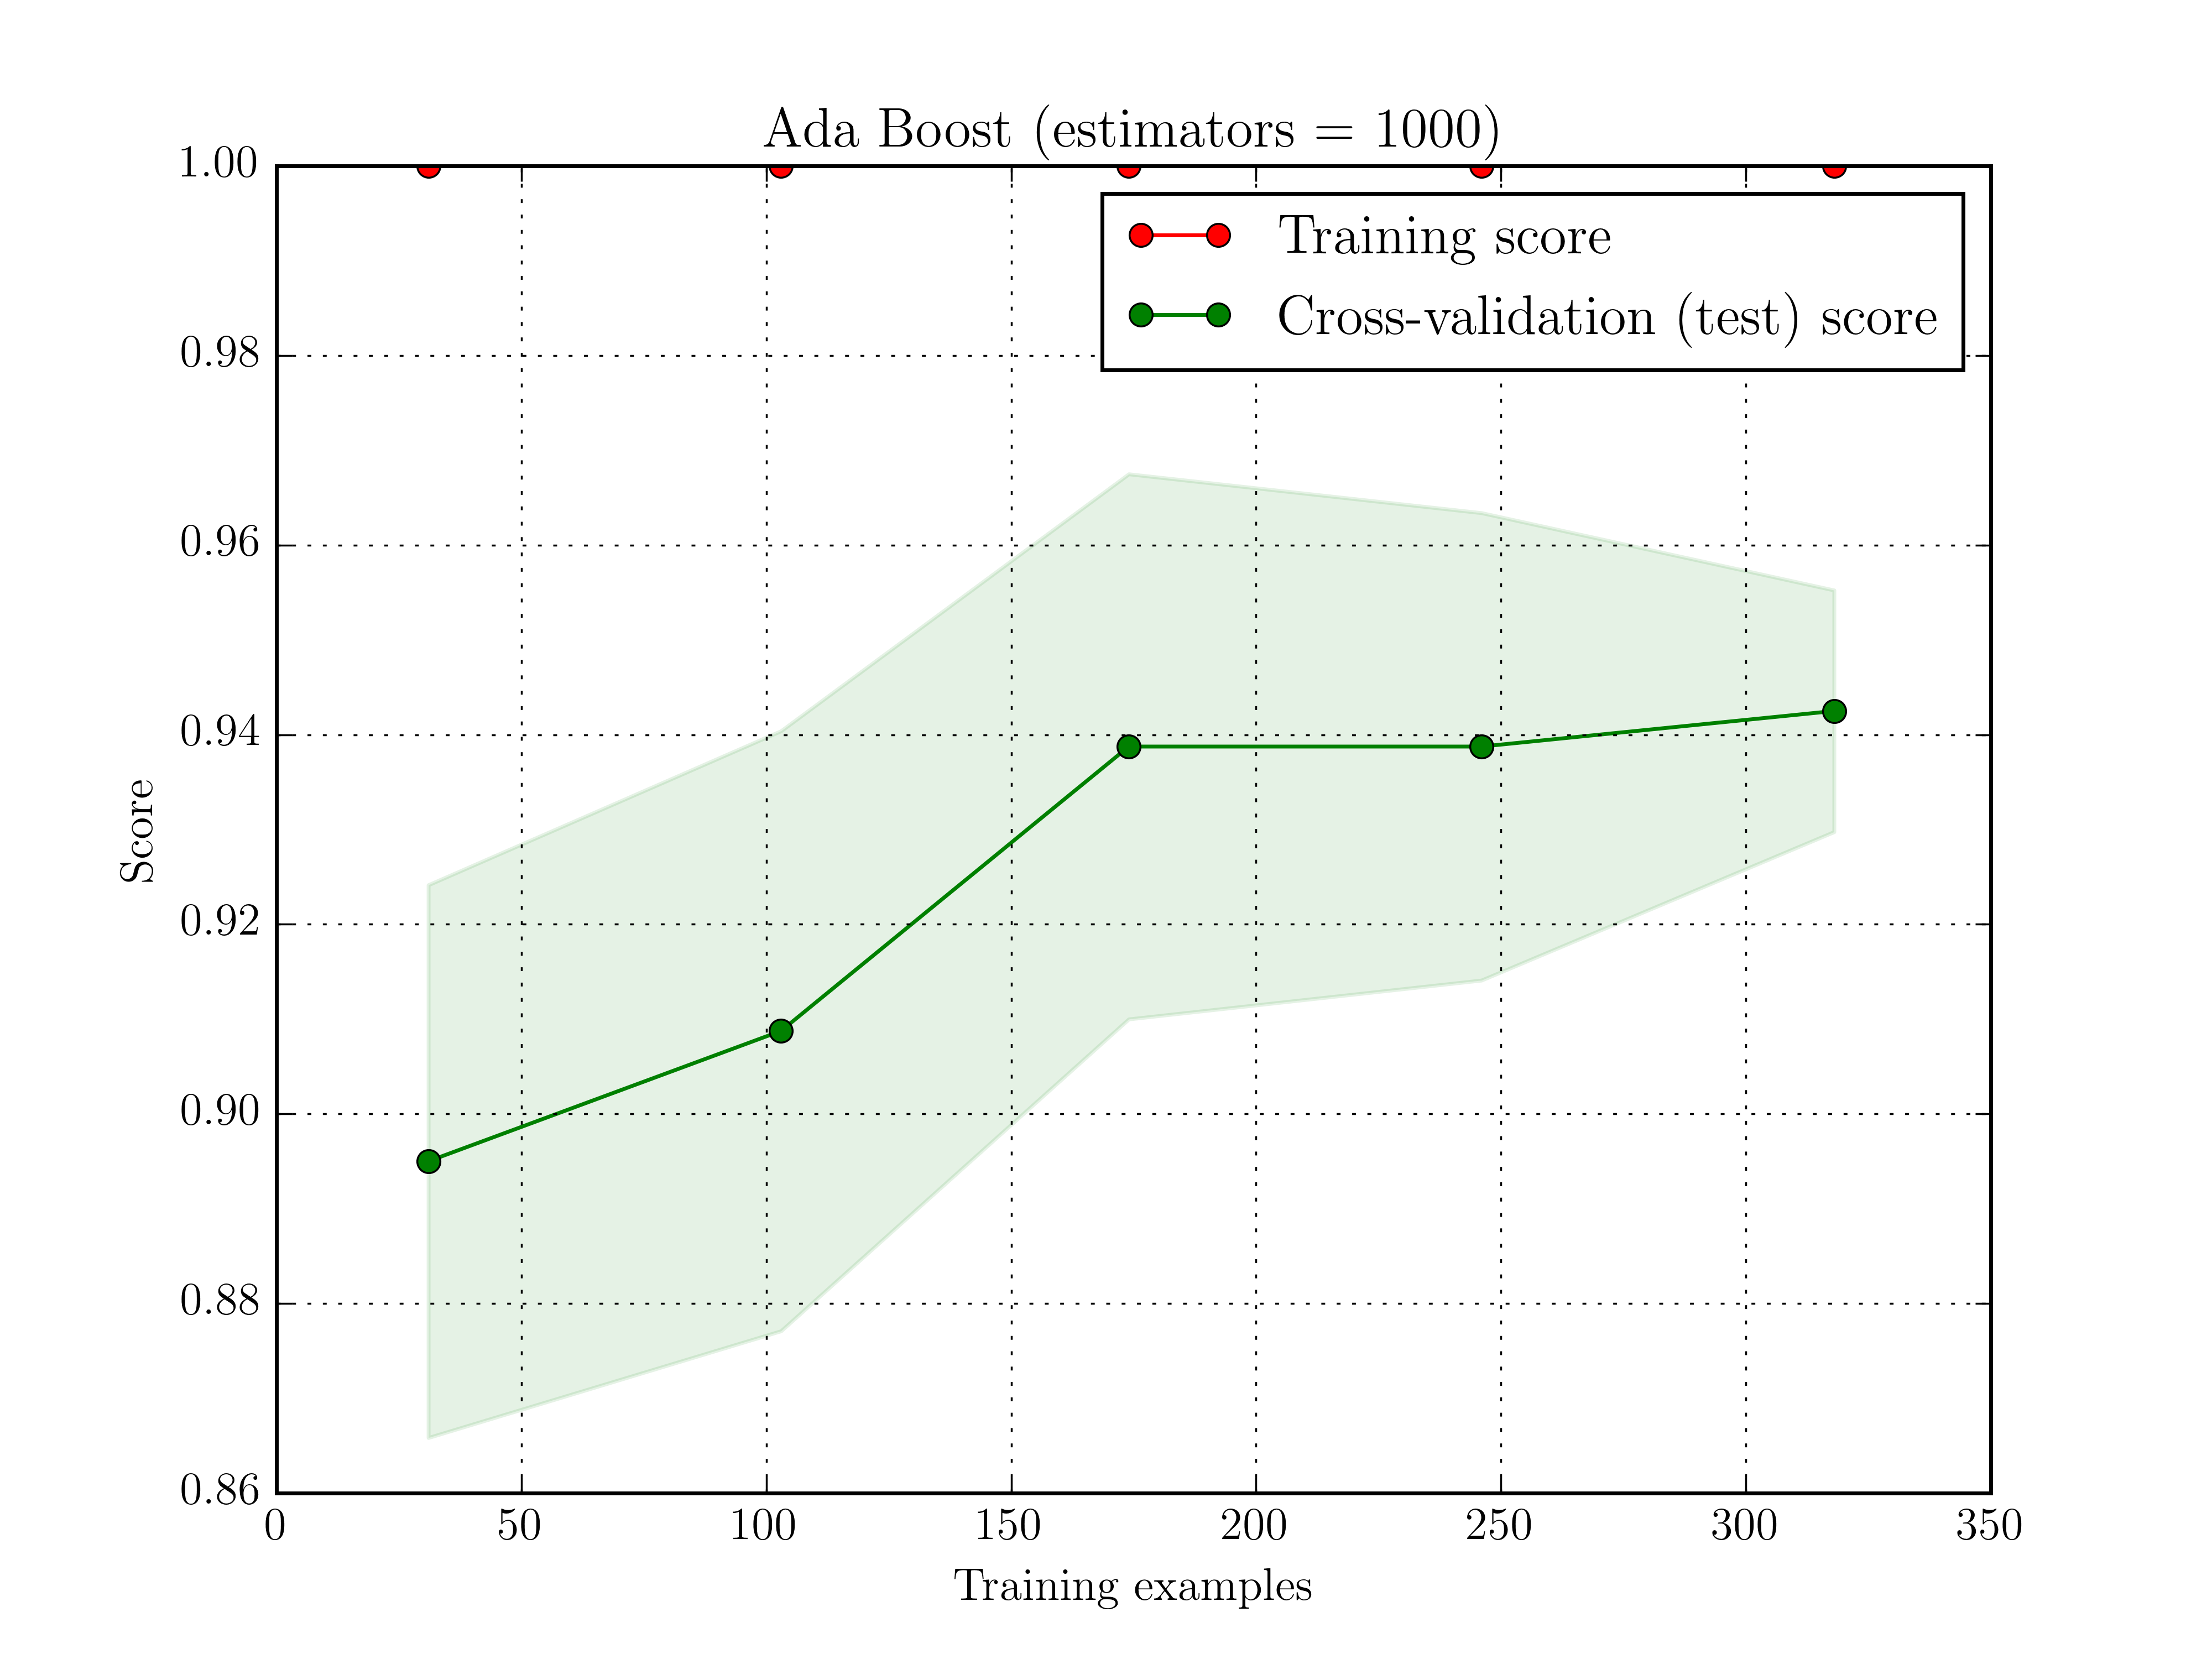
\includegraphics[width=.7\textwidth]{breast/boost.png}
    \caption{AdaBoost with decision tree estimators on breast cancer data set. Runtime: 4 minutes}
\end{figure}

The following is a table for accuracy values for other estimators retrieved from the grid search algorithm.
The most accurate number of estimators (the one that is graphed) is shown in bold.
\begin{center}
    \begin{tabular}{l|| c | c | c | c | c | c | c | c | c | c}
        $k$ = & 37    & 54    & 78    & 112   & 162   & 233   & 335   & 483   & 695   & \textbf{1000}\\
         \hline
         mean & 0.946 & 0.935 & 0.937 & 0.945 & 0.938 & 0.938 & 0.935 & 0.941 & 0.932 & \textbf{0.950}\\
         std  & 0.032 & 0.028 & 0.028 & 0.018 & 0.025 & 0.031 & 0.015 & 0.026 & 0.024 & \textbf{0.022}
    \end{tabular}
\end{center}

Values of \textit{k} were chosen from the set $\{10^{a}$ $|$ $a \in [0, 3]\}$. 20 of theses were selected, with the first $a=0$, the last $a=3$, and the values in between increasing uniformly from 0 to 3 with a step size of $\frac{ln20}{ln10}$. The final value $10^{a}$ was rounded to an integer. This is implemented by the \href{http://docs.scipy.org/doc/numpy-1.10.0/index.html}{\texttt{NumPy}} method \href{http://docs.scipy.org/doc/numpy-1.10.0/reference/generated/numpy.logspace.html}{\texttt{logspace}}.

\subsection{\textit{k}-nearest neighbors}
\begin{figure}[H]
    \centering
    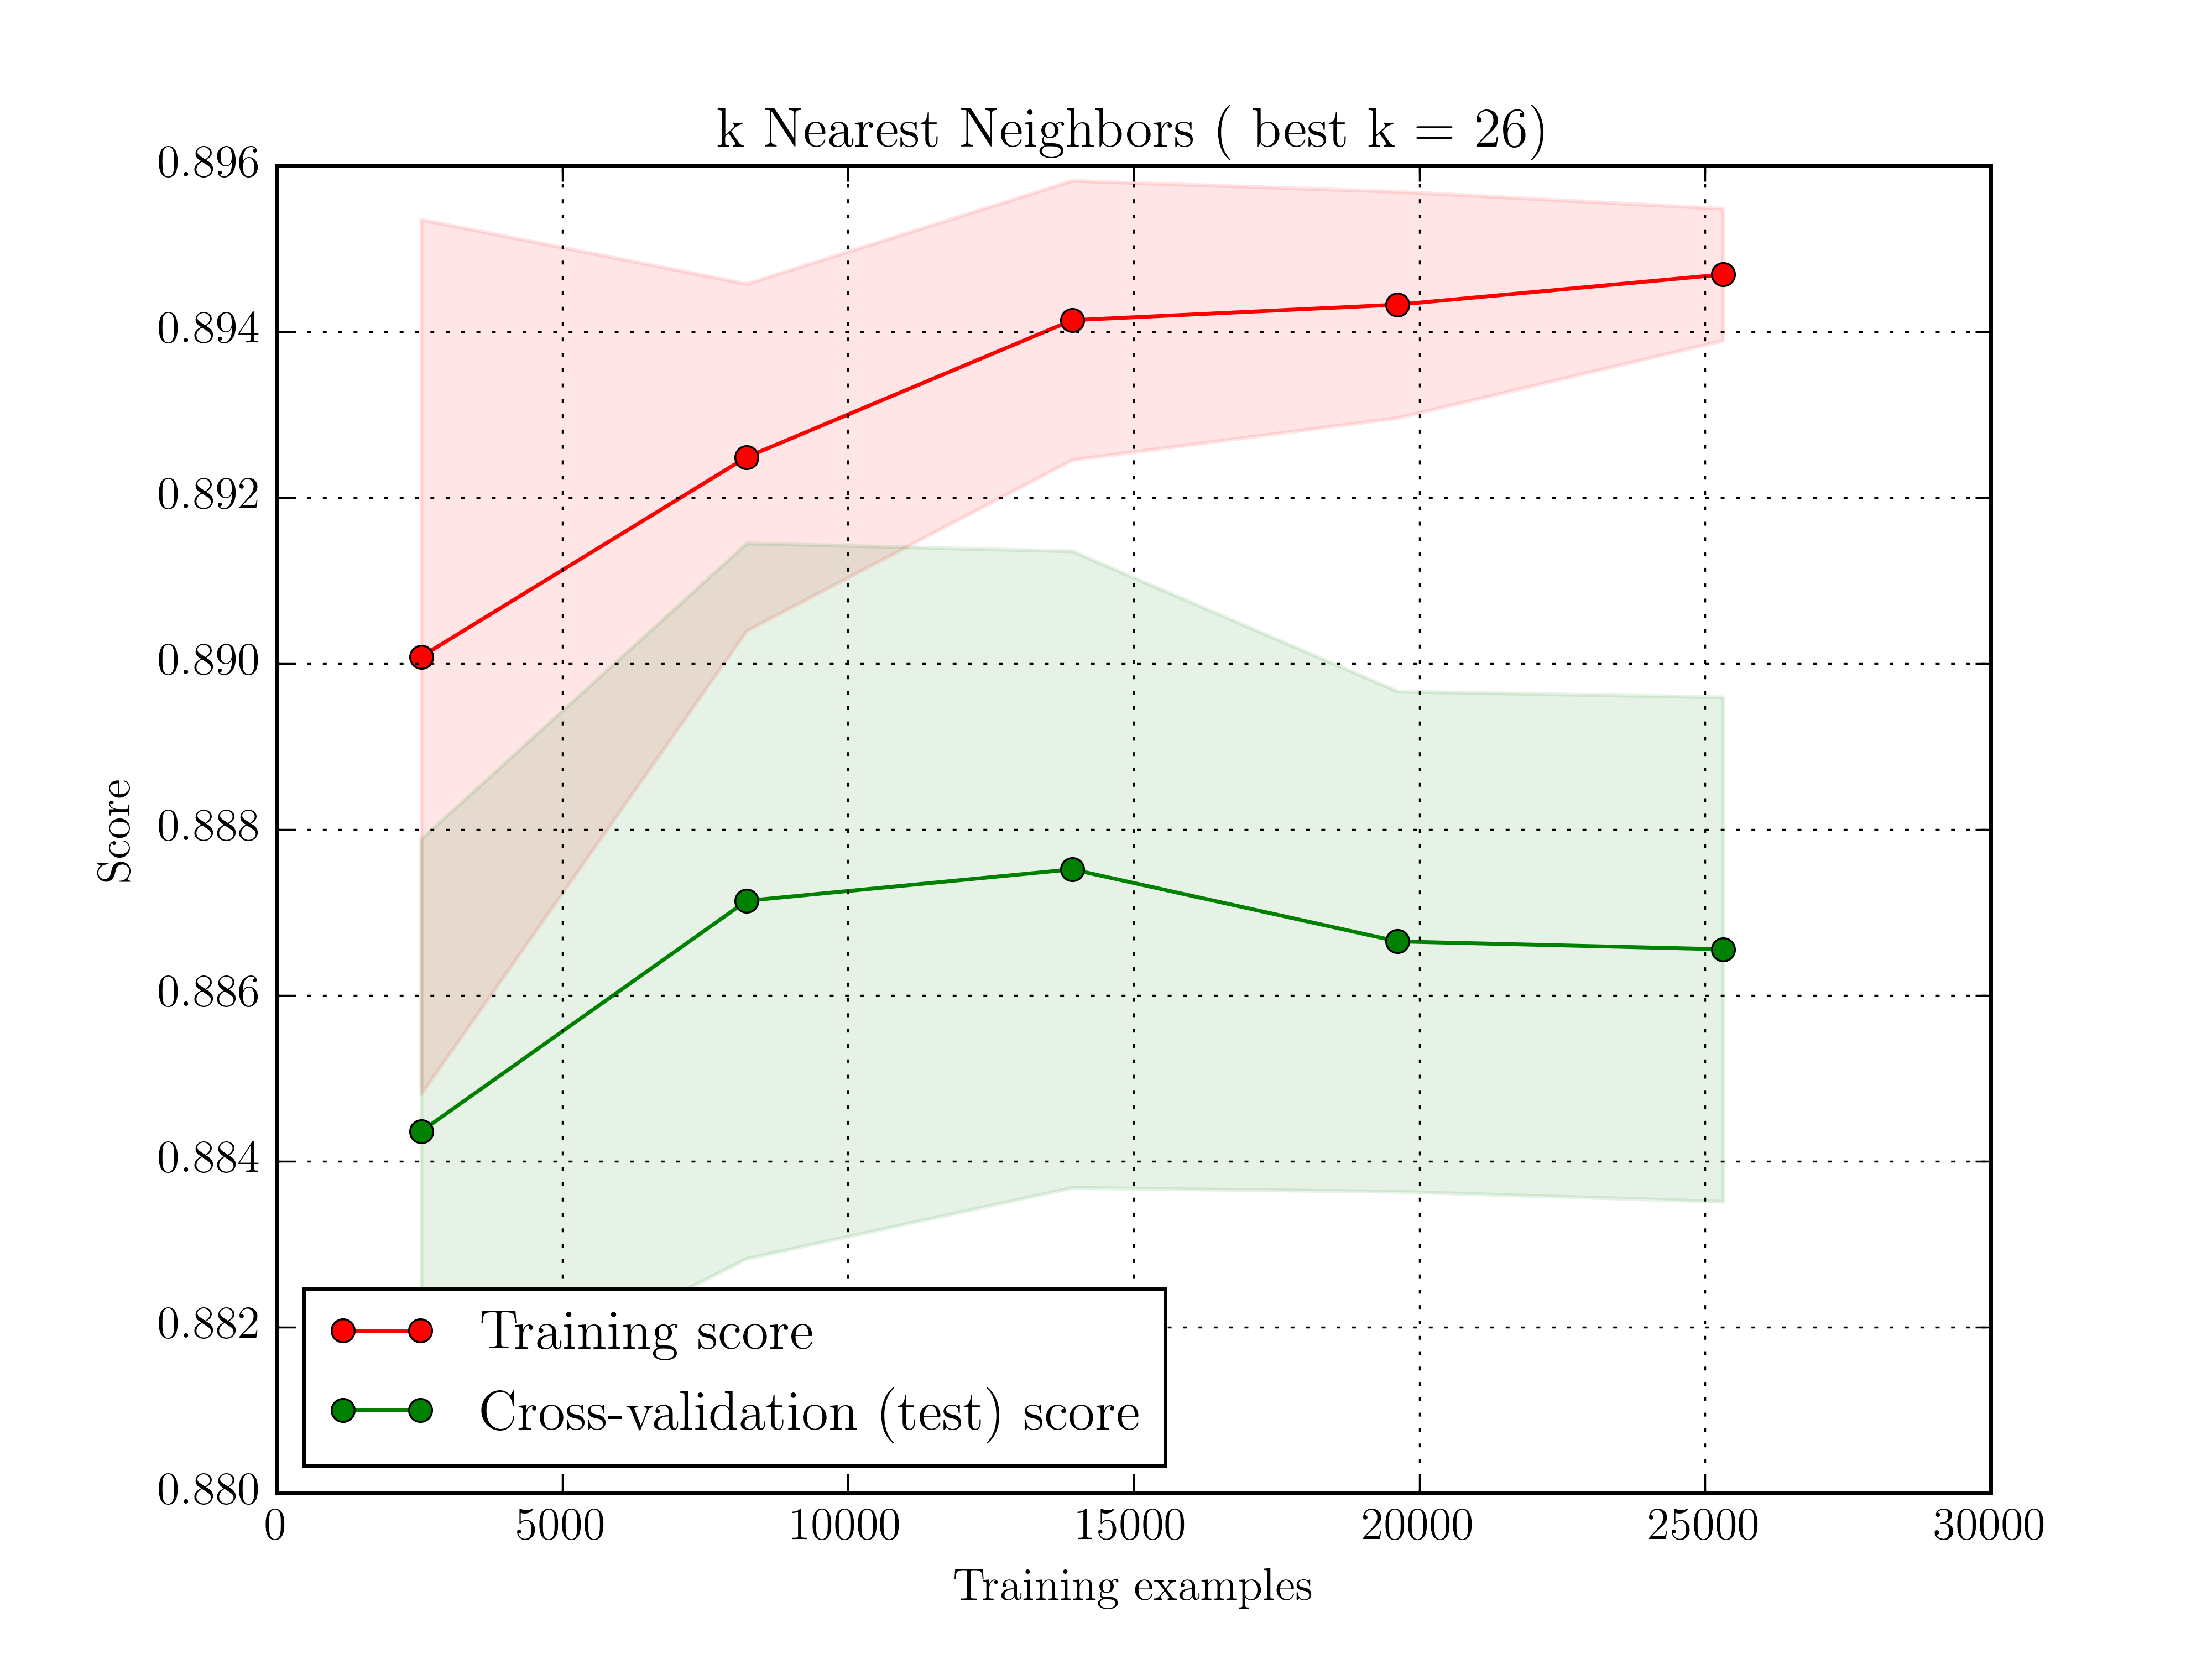
\includegraphics[width=.7\textwidth]{bank/knn.png}
    \caption{$k$-nearest neighbors on bank marketing data set. Runtime: 3 minutes}
\end{figure}

The following is a table for accuracy values for other \textit{k} retrieved from the grid search algorithm.
The most accurate \textit{k} (the one that is graphed) is shown in bold.
\begin{center}
    \begin{tabular}{l|| c | c | c | c | c | c | c | c | c | c}
        $k$ = & 6     & 7     & 8     & 10    & 12    & 15    & 18    & 21    & \textbf{26}    & 31\\
         \hline
         mean & 0.880 & 0.884 & 0.884 & 0.886 & 0.887 & 0.888 & 0.888 & 0.887 & \textbf{0.890} & 0.888\\
         std  & 0.004 & 0.002 & 0.004 & 0.003 & 0.003 & 0.003 & 0.002 & 0.002 & \textbf{0.004} & 0.002
    \end{tabular}
\end{center}

\begin{figure}[H]
    \centering
    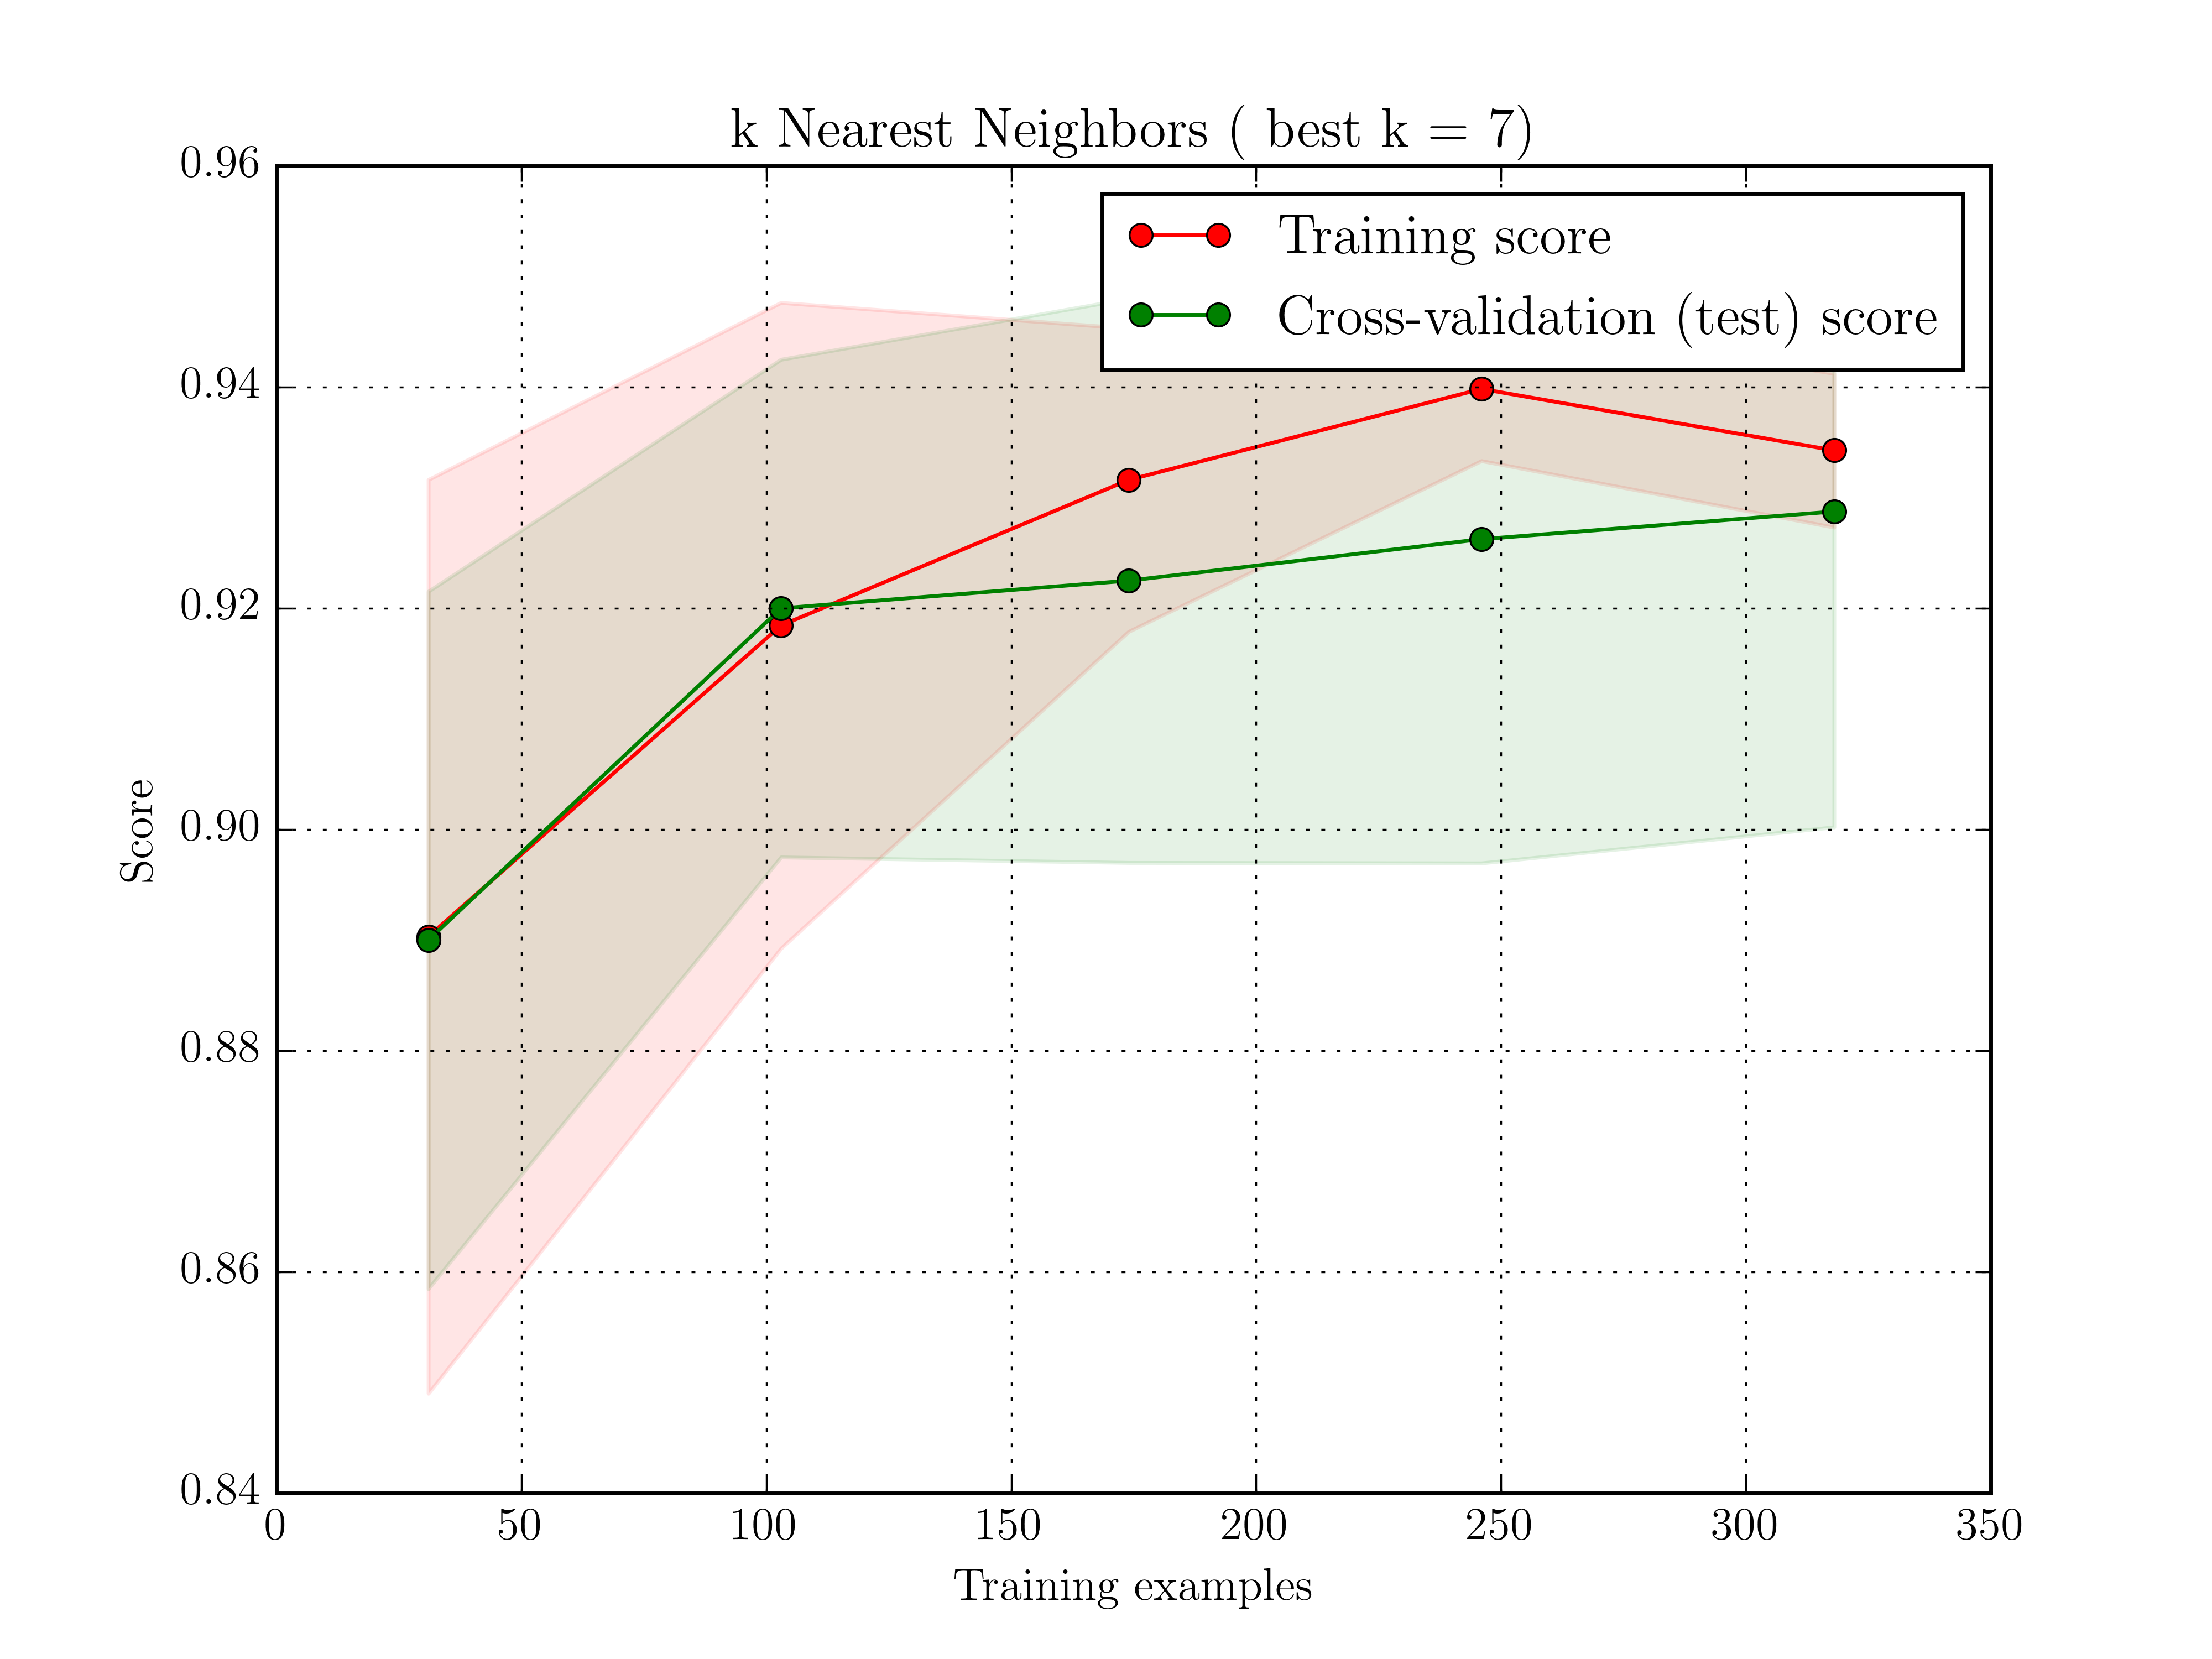
\includegraphics[width=.7\textwidth]{breast/knn.png}
    \caption{$k$-nearest neighbors on breast cancer data set. Runtime: 3 seconds}
\end{figure}

The following is a table for accuracy values for other \textit{k} retrieved from the grid search algorithm.
The most accurate \textit{k} (the one that is graphed) is shown in bold.

\begin{center}
    \begin{tabular}{l|| c | c | c | c | c | c | c | c | c | c}
        $k$ = & 1     & 2     & 3     & 4     & 5     & 6     & \textbf{7}     & 8     & 10    & 12\\
         \hline
         mean & 0.913 & 0.902 & 0.936 & 0.925 & 0.920 & 0.911 & \textbf{0.938} & 0.915 & 0.930 & 0.906\\
         std  & 0.042 & 0.015 & 0.024 & 0.024 & 0.030 & 0.029 & \textbf{0.022} & 0.040 & 0.021 & 0.024
    \end{tabular}
\end{center}

Values of \textit{k} were chosen from the set $\{10^{a}$ $|$ $a \in [0, 1.5]\}$. 20 of theses were selected, with the first $a=0$, the last $a=1.5$, and the values in between increasing uniformly from 0 to 1.5 with a step size of $\frac{ln20}{ln10}$. The final value $10^{a}$ was rounded to an integer. This is implemented by the \href{http://docs.scipy.org/doc/numpy-1.10.0/index.html}{\texttt{numpy}} method \href{http://docs.scipy.org/doc/numpy-1.10.0/reference/generated/numpy.logspace.html}{\texttt{logspace}}.

\subsection{Decision tree}

\begin{figure}[H]
    \centering
    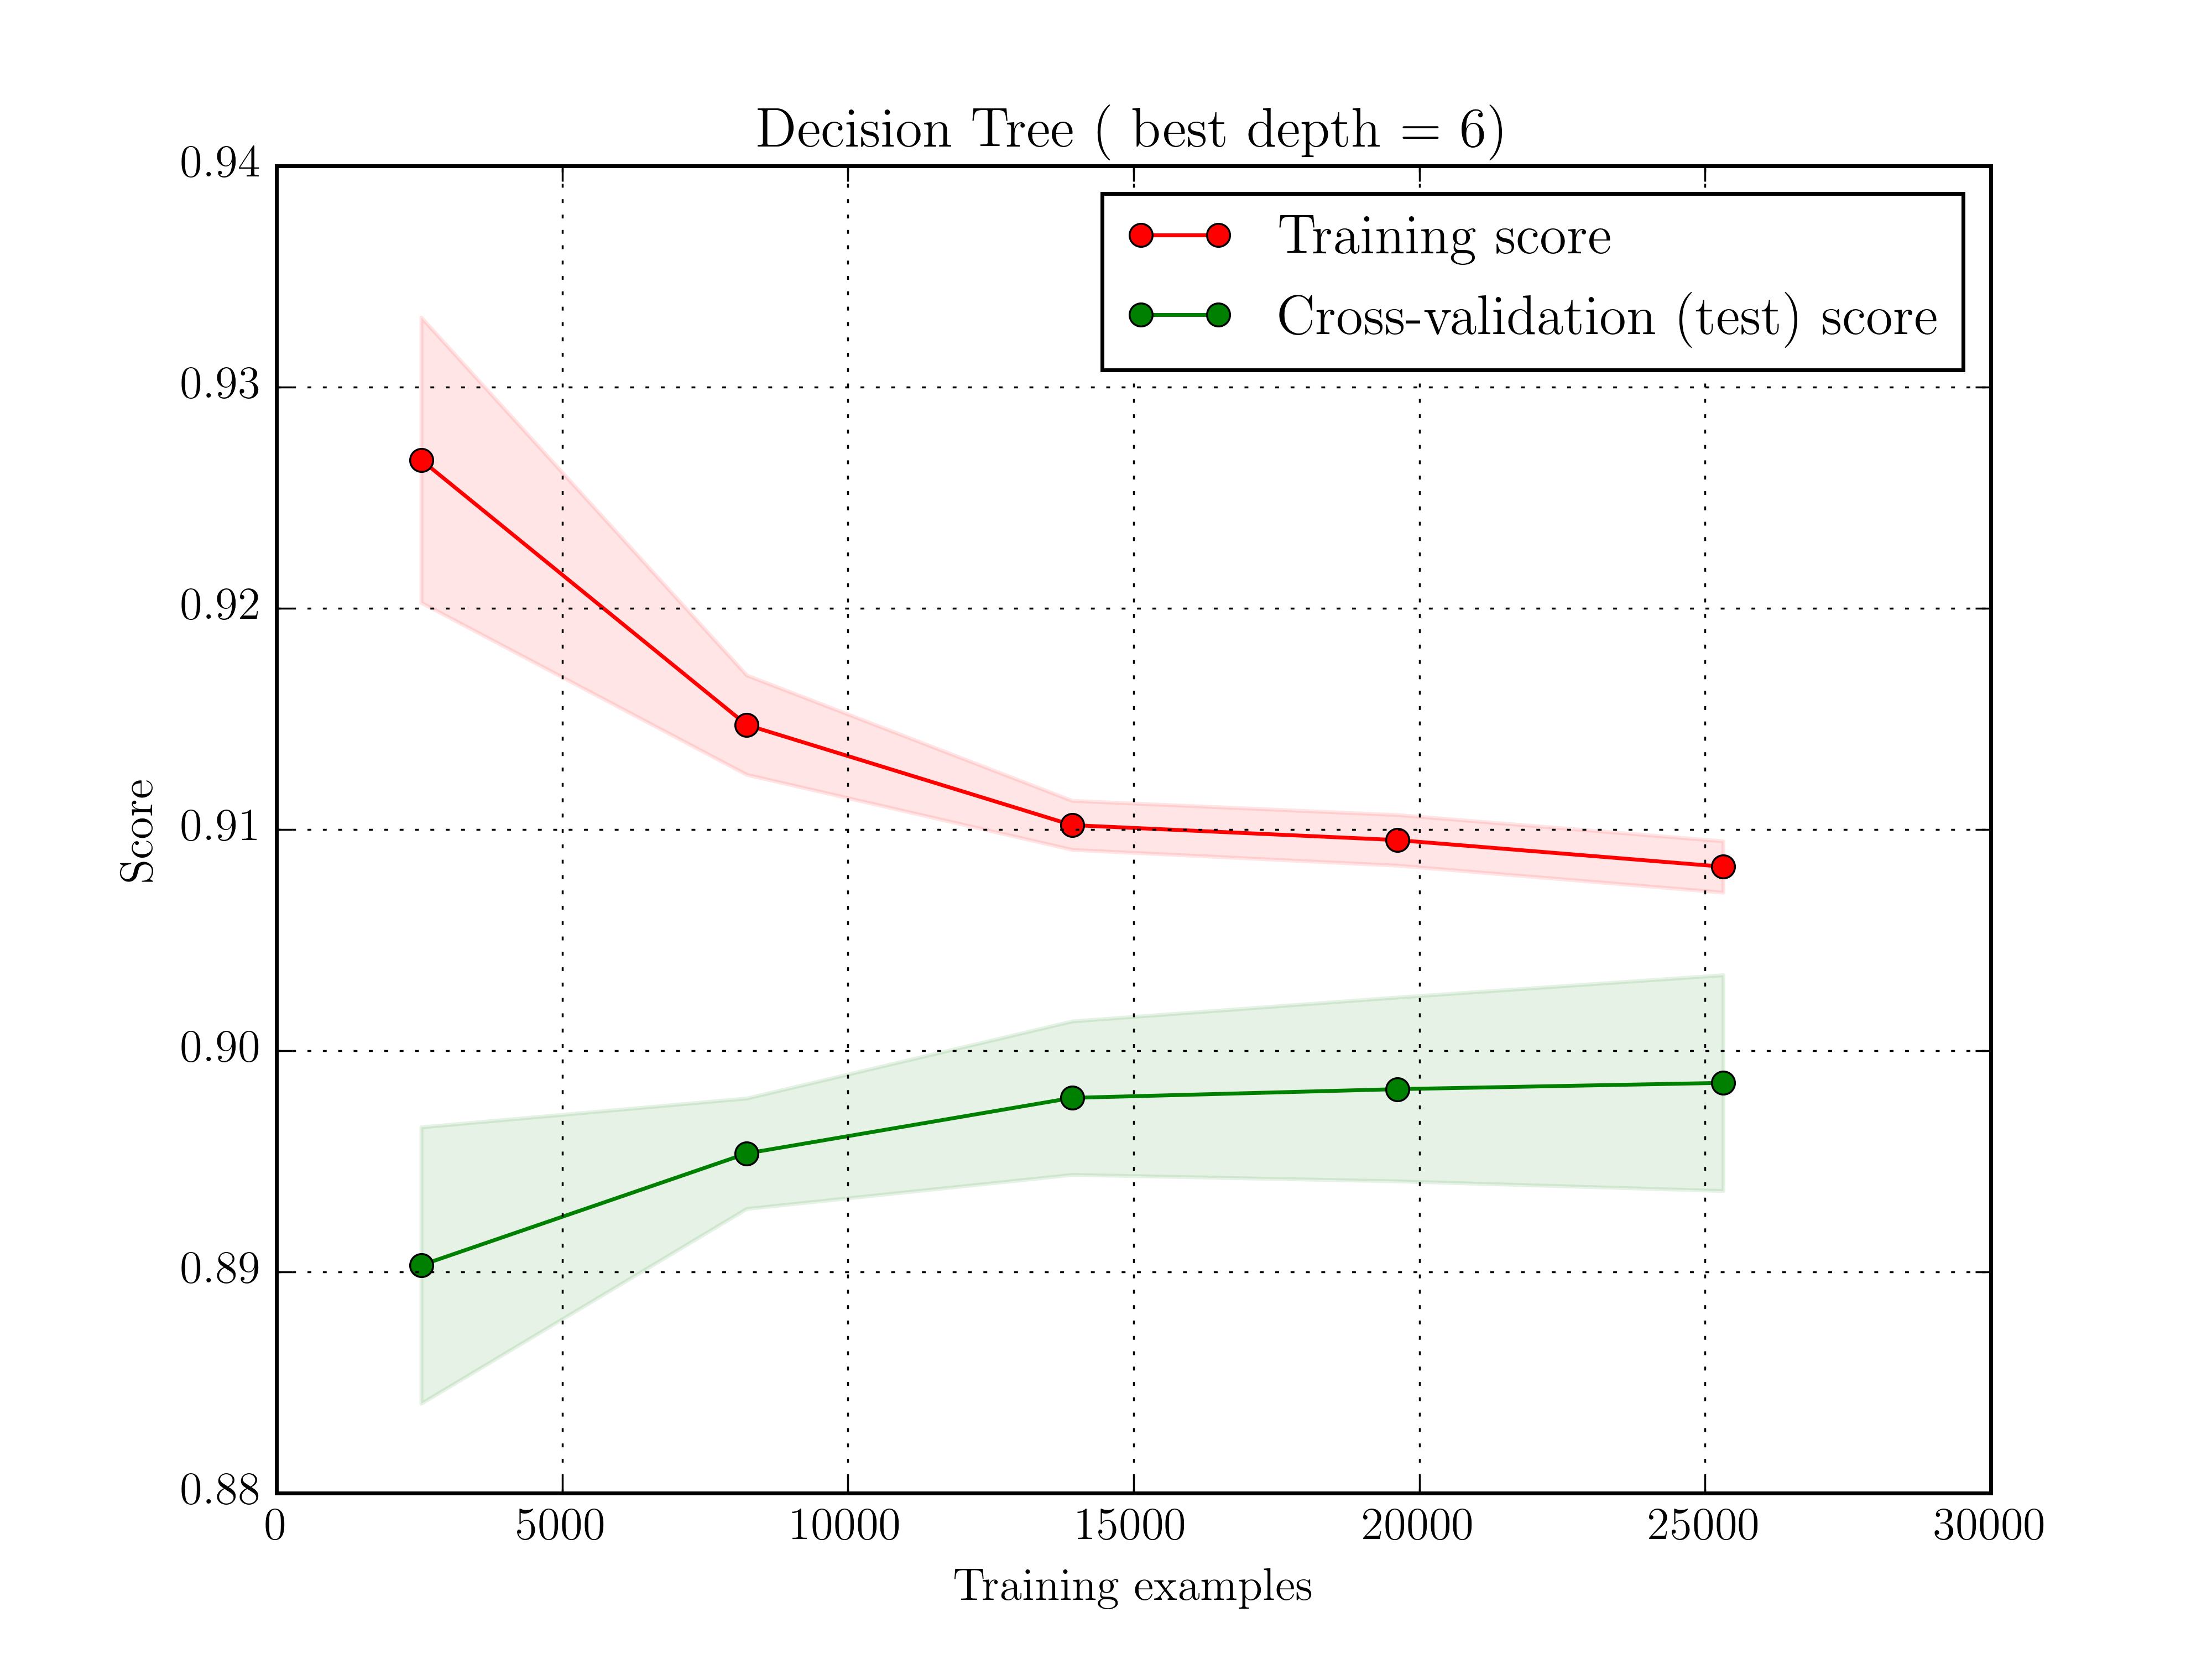
\includegraphics[width=.7\textwidth]{bank/tree.png}
    \caption{Decision tree on bank marketing data set. Runtime: 10 minutes}
\end{figure}
The following is a table for accuracy values for other depths retrieved from the grid search algorithm.
The most accurate depth (the one that is graphed) is shown in bold.
\begin{center}
    \begin{tabular}{l|| c | c | c | c | c | c | c | c | c | c}
        $k$ = & 2     & 3     & 4     & 5     & \textbf{6}     & 7     & 8     & 9     & 10    & 11\\
         \hline
         mean & 0.895 & 0.901 & 0.900 & 0.899 & \textbf{0.902} & 0.898 & 0.899 & 0.898 & 0.896 & 0.894\\
         std  & 0.003 & 0.002 & 0.002 & 0.001 & \textbf{0.004} & 0.003 & 0.003 & 0.002 & 0.003 & 0.004
    \end{tabular}
\end{center}

The following is a table of the weights the decision tree algorithm gave for the attributes.
\begin{center}
    \begin{tabular}{|l|l|}
        \hline
        age:       0.0407 & contact:  0.0223\\
        job:       0.0053 & day:      0.0027\\
        marital:   0.0058 & month:    0.0206\\
        education: 0      & duration: 0.5228\\
        default:   0      & campaign: 0.0012\\
        balance:   0.0046 & pdays:    0.0368\\
        housing:   0.0450 & previous: 0.0017\\
        loan:      0      & poutcome: 0.2900\\
        \hline
    \end{tabular}
\end{center}

\begin{figure}[H]
    \centering
    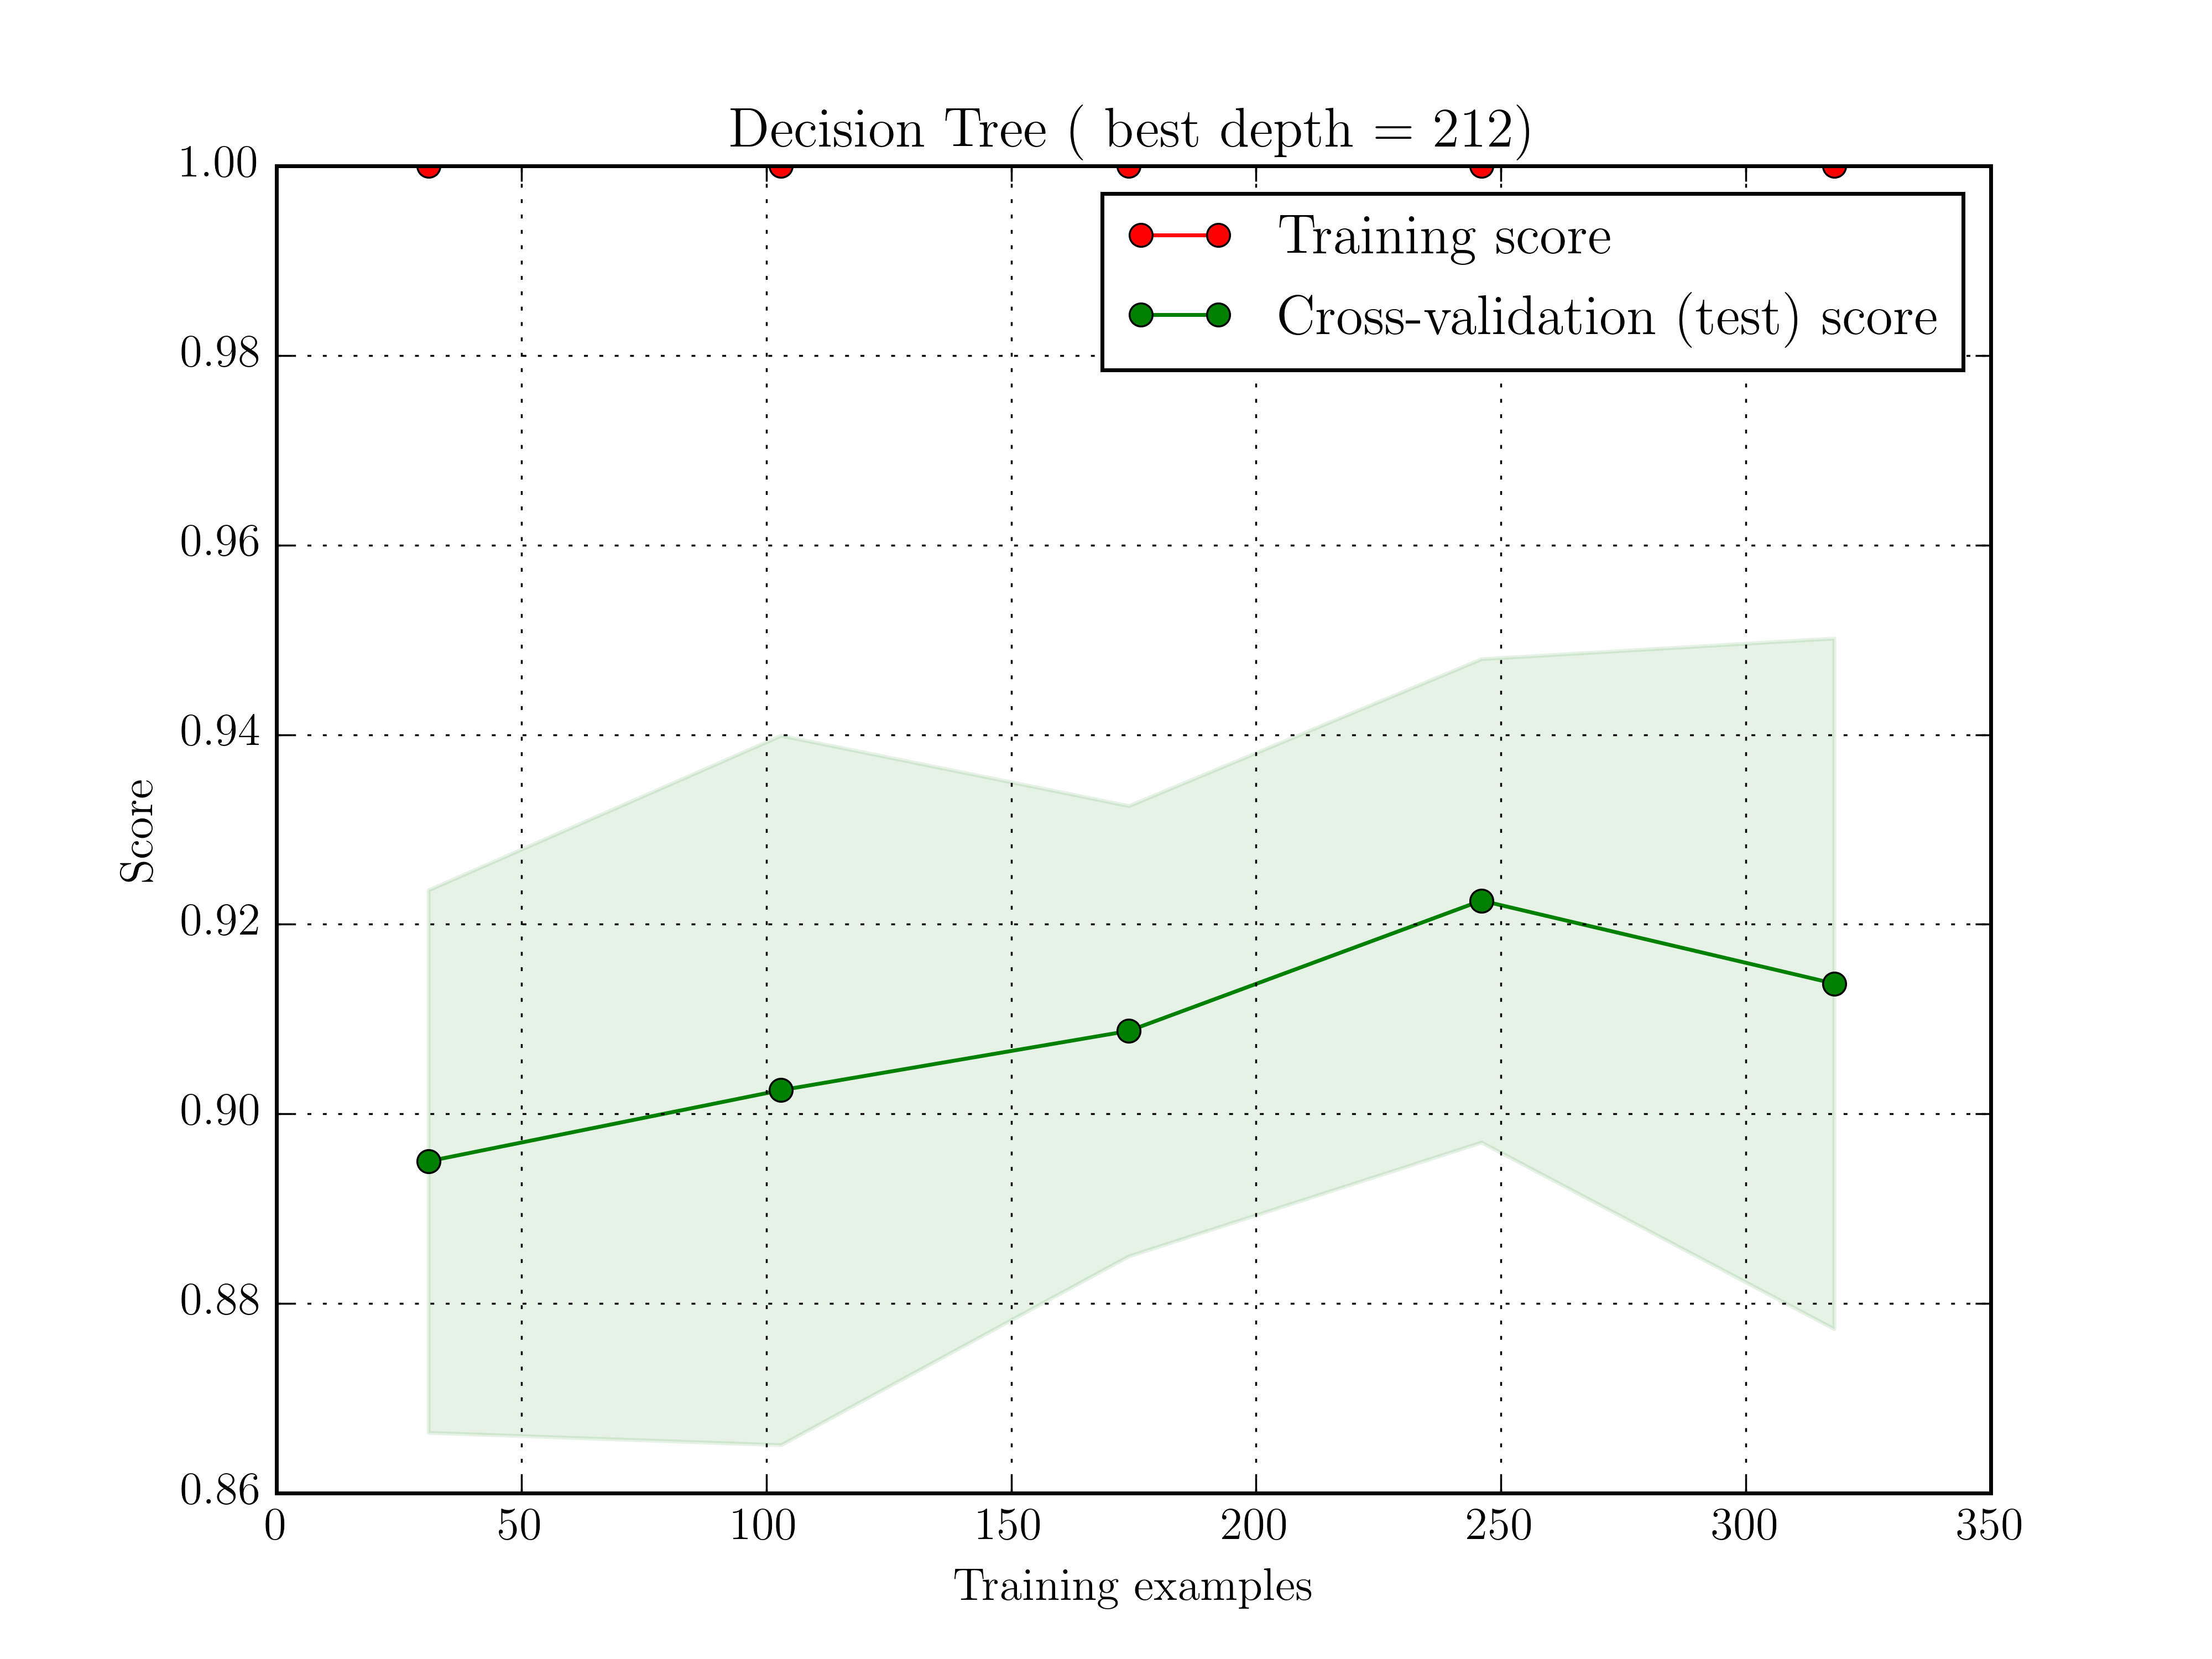
\includegraphics[width=.7\textwidth]{breast/tree.png}
    \caption{Decision tree on breast cancer data set. Runtime: 16 seconds}
\end{figure}

The following is a table for accuracy values for other depths retrieved from the grid search algorithm.
The most accurate depth (the one that is graphed) is shown in bold.
\begin{center}
    \begin{tabular}{l|| c | c | c | c | c | c | c | c | c | c}
        $k$ = & 208   & 209   & 210   & 211   & \textbf{212}   & 213   & 214   & 215   & 216   & 217\\
         \hline
         mean & 0.917 & 0.907 & 0.901 & 0.905 & \textbf{0.933} & 0.908 & 0.907 & 0.907 & 0.921 & 0.932\\
         std  & 0.028 & 0.029 & 0.030 & 0.030 & \textbf{0.015} & 0.019 & 0.021 & 0.031 & 0.020 & 0.025
    \end{tabular}
\end{center}

The following is a table of the weights the decision tree algorithm gave for the attributes.
\begin{center}
    \begin{tabular}{l||l|l|l}
                          & mean      & standard error & worst\\
        \hline
        radius            & 0.033791  & 0              & 0\\
        texture           & 0.067506  & 0.001769       & 0.033169\\
        perimeter         & 0.015582  & 0              & 0.779885\\
        area              & 0.026663  & 0.018520       & 0.012741\\
        smoothness        & 0         & 0              & 0\\
        compactness       & 0         & 0              & 0.010370\\
        concavity         & 0         & 0              & 0\\ 
        concave points    & 0         & 0              & 0\\
        symmetry          & 0         & 0              & 0\\
        fractal dimension & 0         & 0              & 0\\
    \end{tabular}
\end{center}

Depths were chosen from the interval [1, 300) with a step size of 1 (i.e. 1, 2, 3 ... 299).

\subsection{Neural network}

\begin{figure}[H]
    \centering
    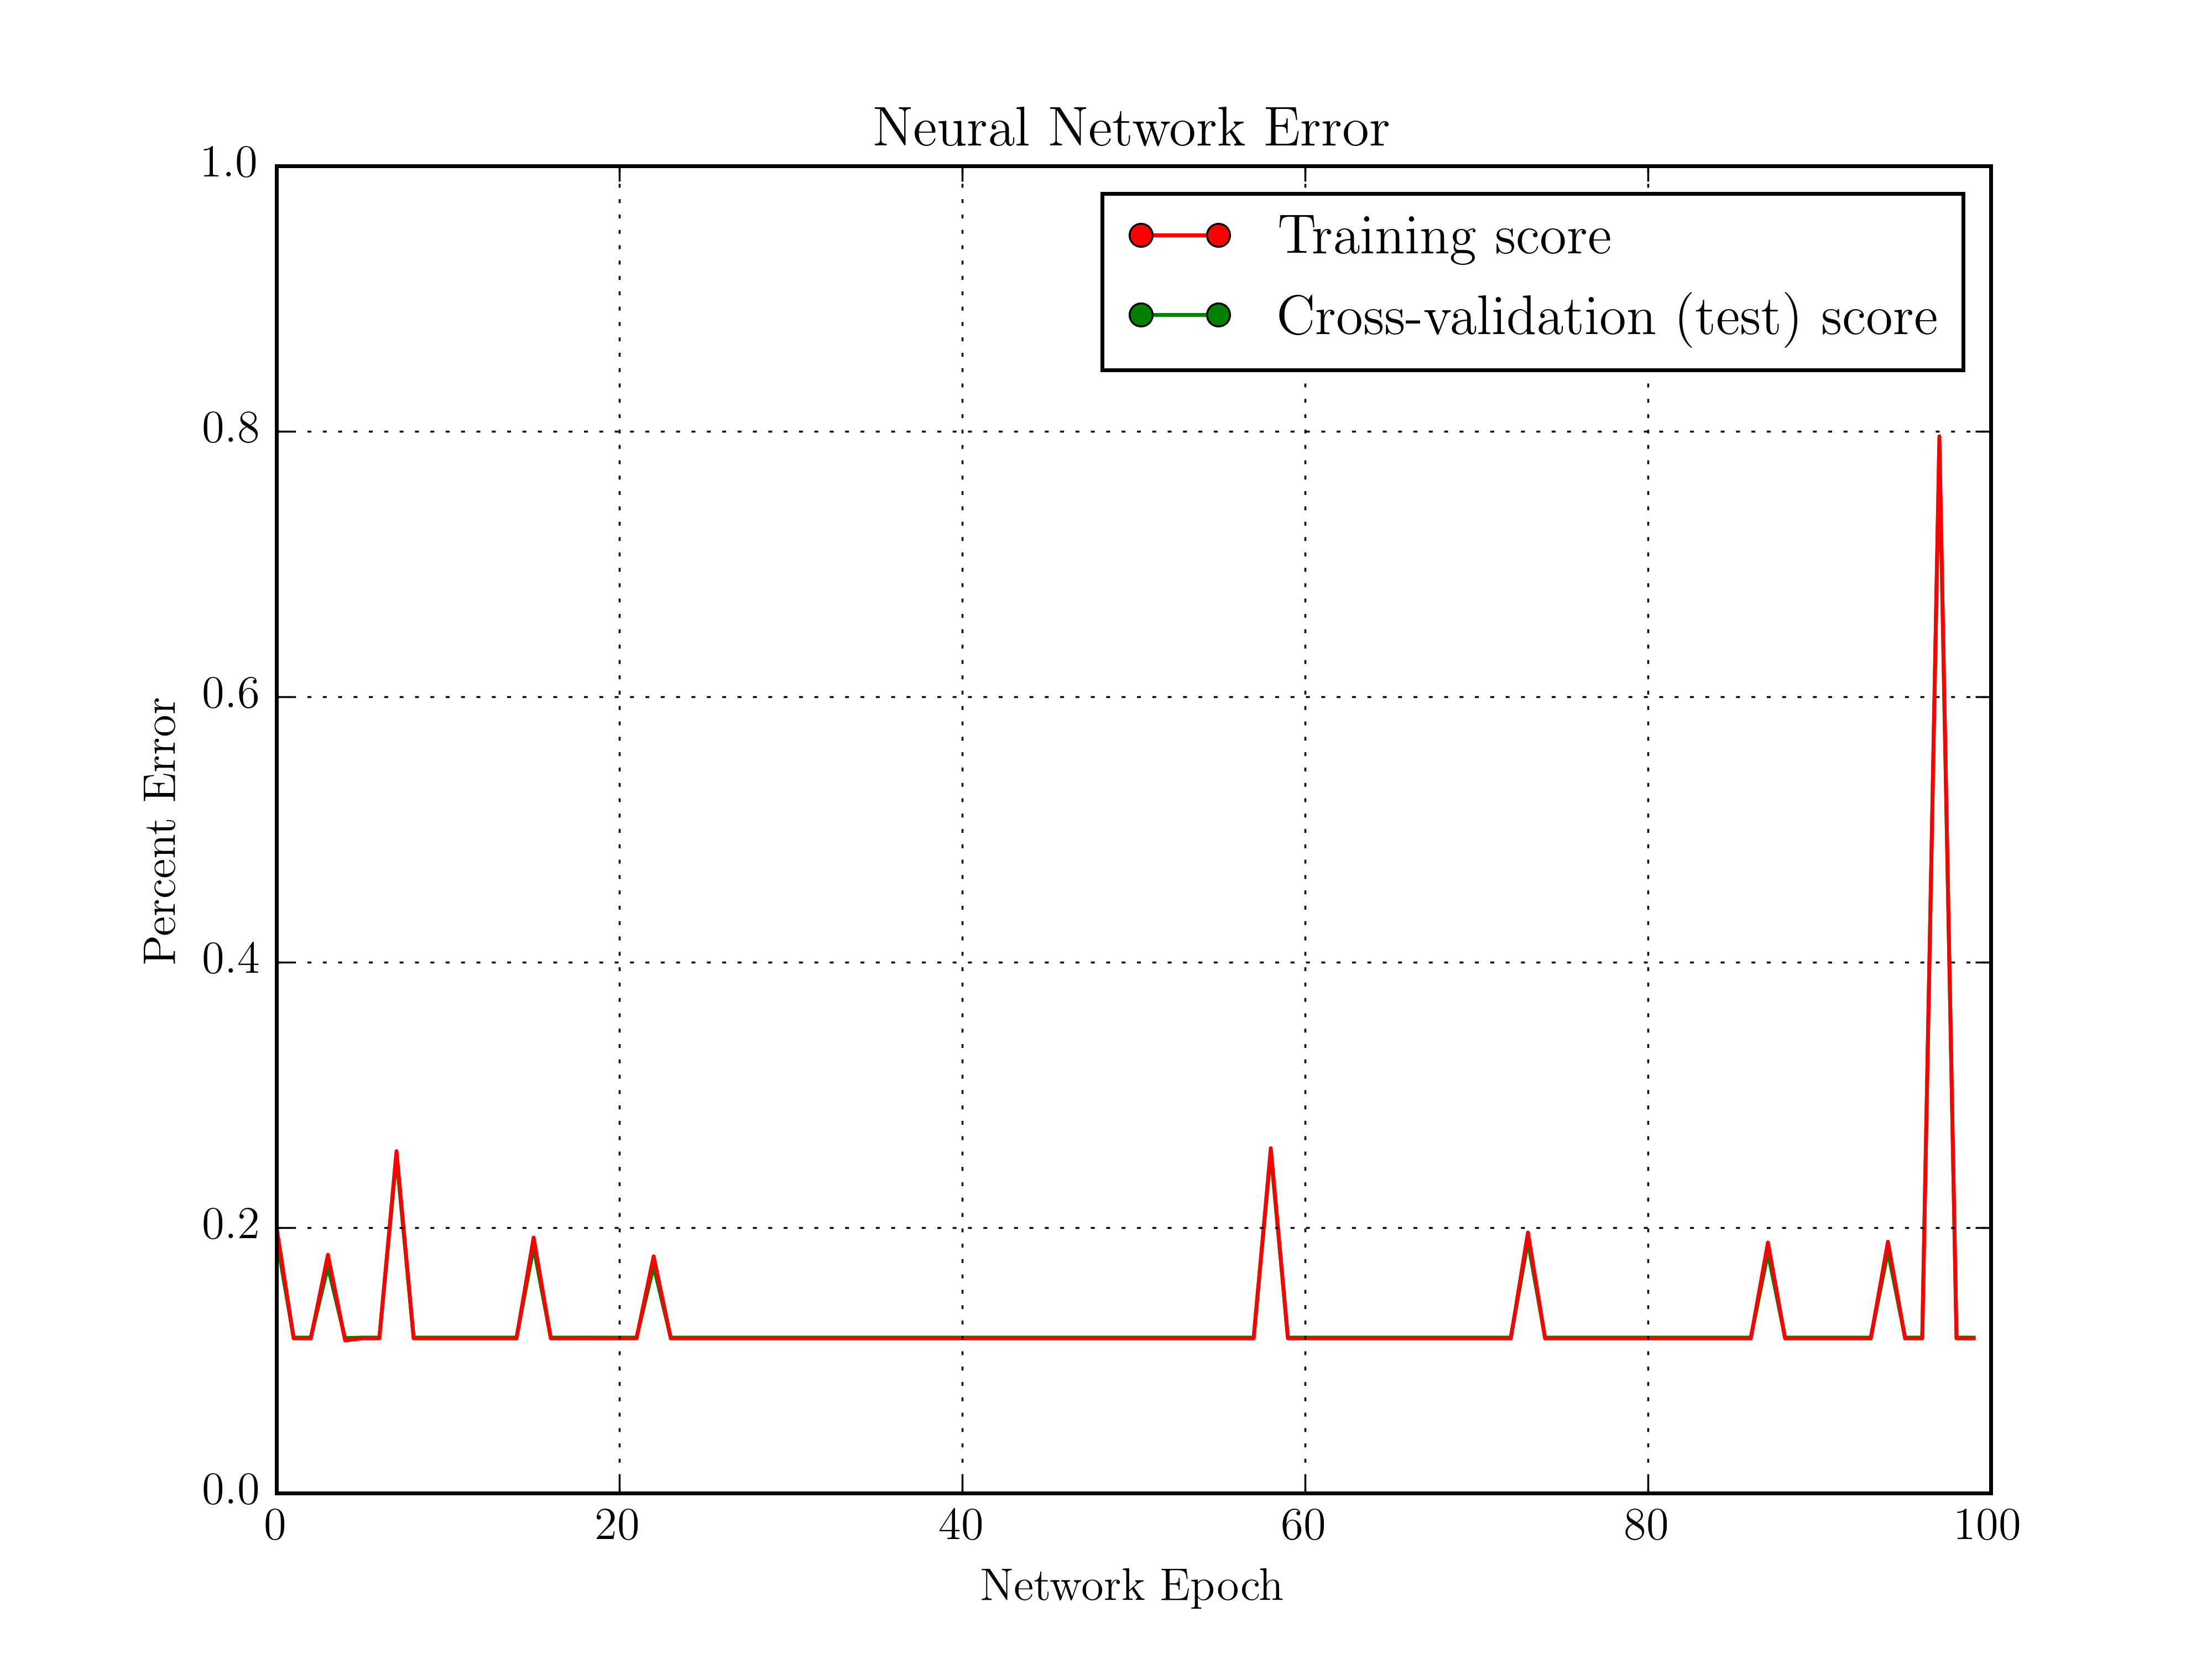
\includegraphics[width=.7\textwidth]{bank/nn.png}
    \caption{Neural network on bank marketing data set (note the complete overlap). Note that this graph measures percentage error, unlike the others. Runtime: 50 minutes}
\end{figure}

\begin{figure}[H]
    \centering
    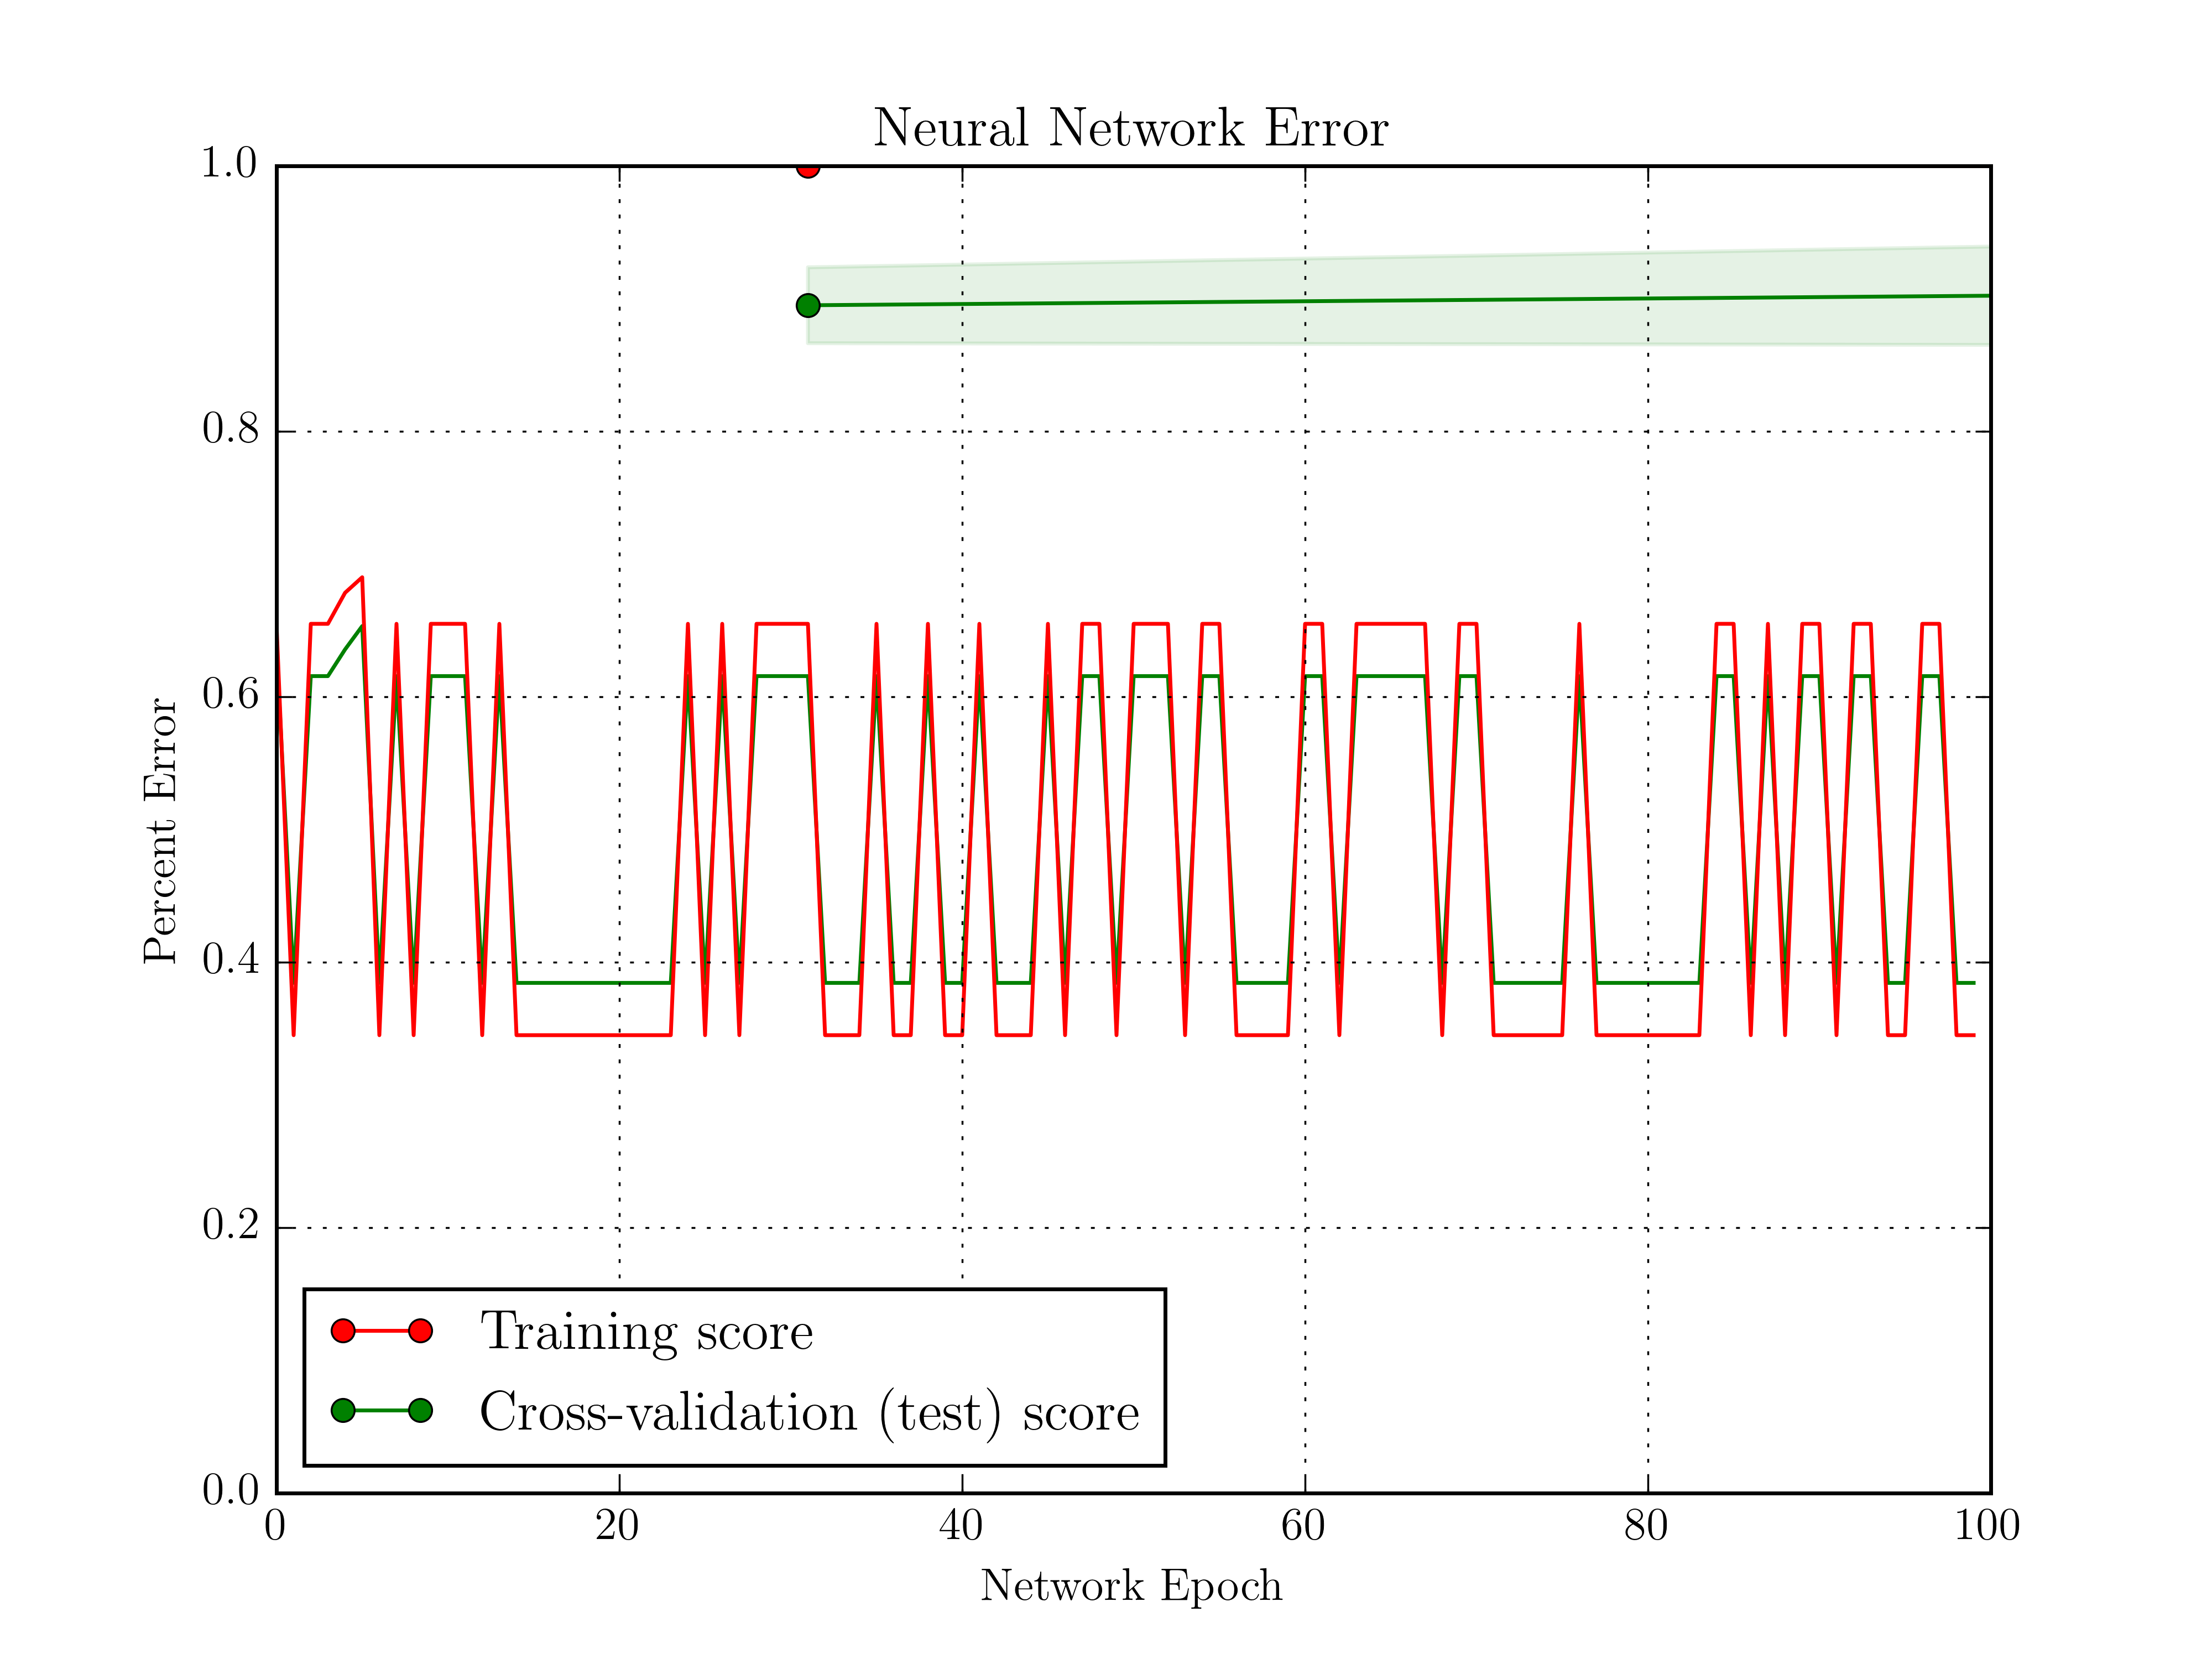
\includegraphics[width=.7\textwidth]{breast/nn.png}
    \caption{Neural network on breast cancer data set (note the complete overlap). Please disregard the two lines in the top right. These are artefacts of of a mis-configuration. Note that this graph measures percentage error, unlike the others. Runtime: 1 minute}
\end{figure}

\subsection{Support vector machine}

\begin{figure}[H]
    \centering
    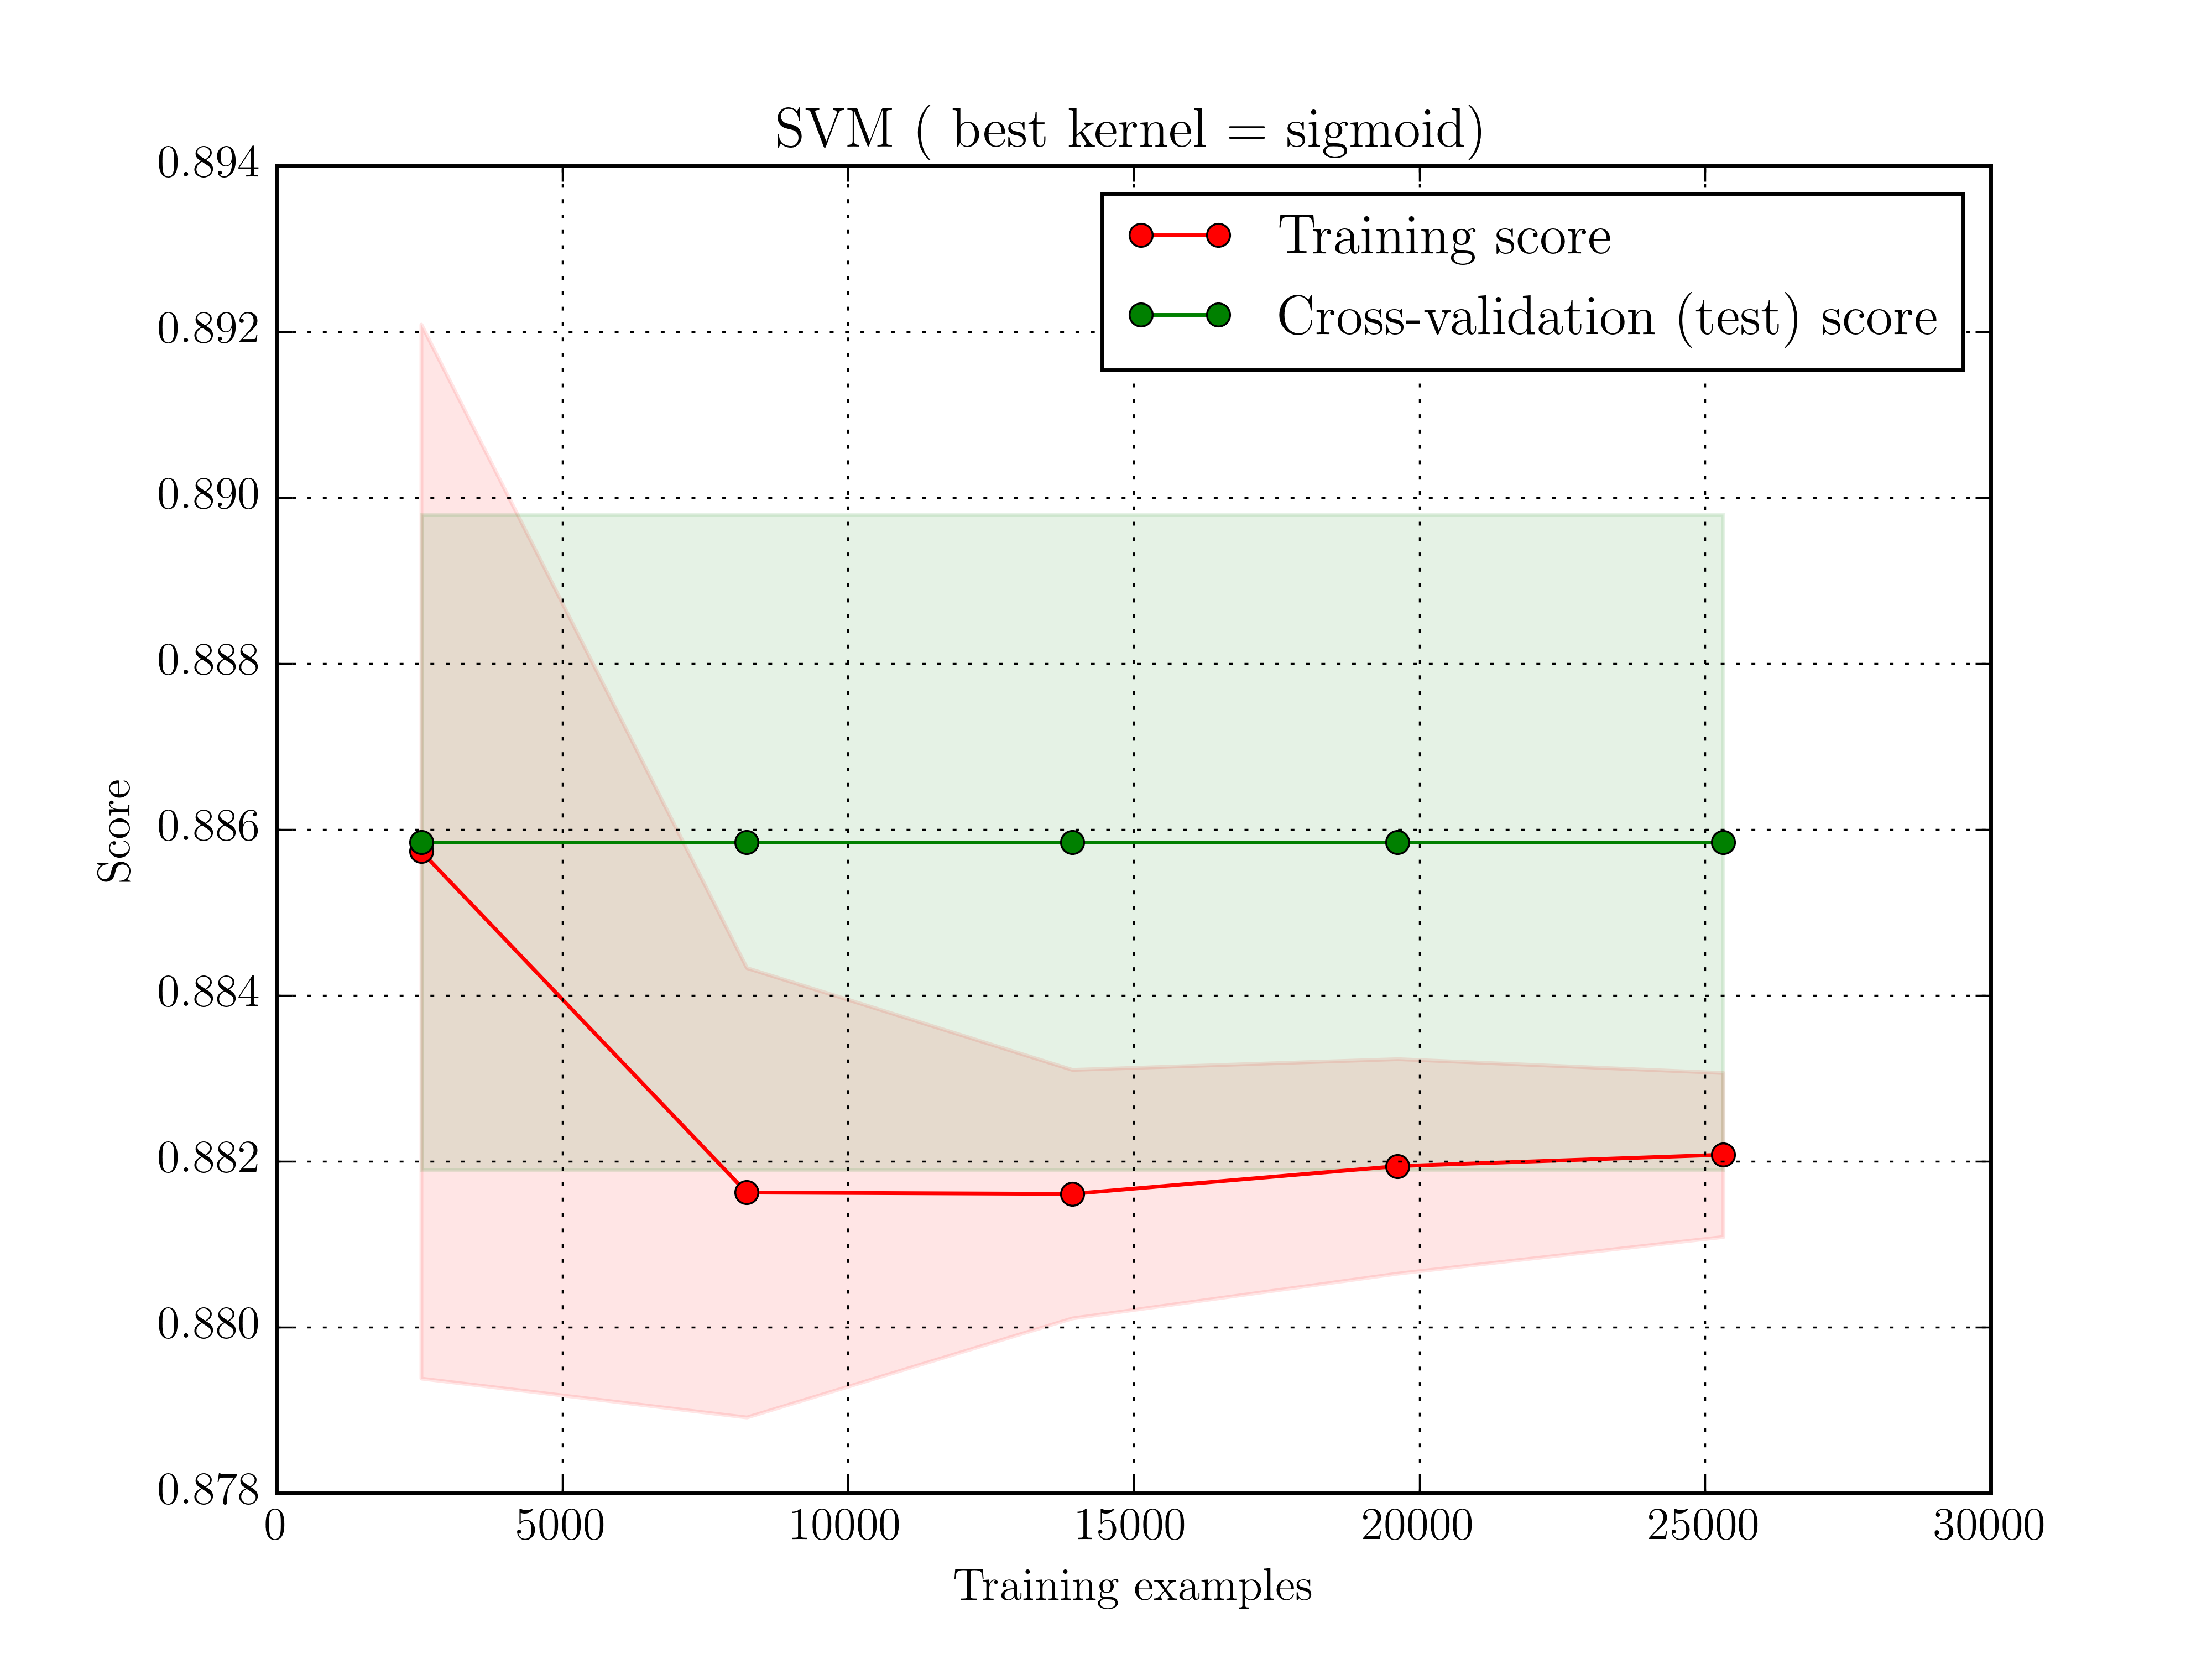
\includegraphics[width=.7\textwidth]{bank/svm.png}
    \caption{SVM on bank marketing data set. Runtime: 12 minutes}
\end{figure}

The following is a table for accuracy values for other kernels retrieved from the grid search algorithm.
The most accurate kernel (the one that is graphed) is shown in bold.
\begin{center}
    \begin{tabular}{l || l | l}
         kernel = & \textbf{sigmoid} & radial basis function\\
         \hline
         mean     & \textbf{0.884}   & 0.882\\
         std      & \textbf{0.002}   & 0.002
    \end{tabular}
\end{center}

\begin{figure}[H]
    \centering
    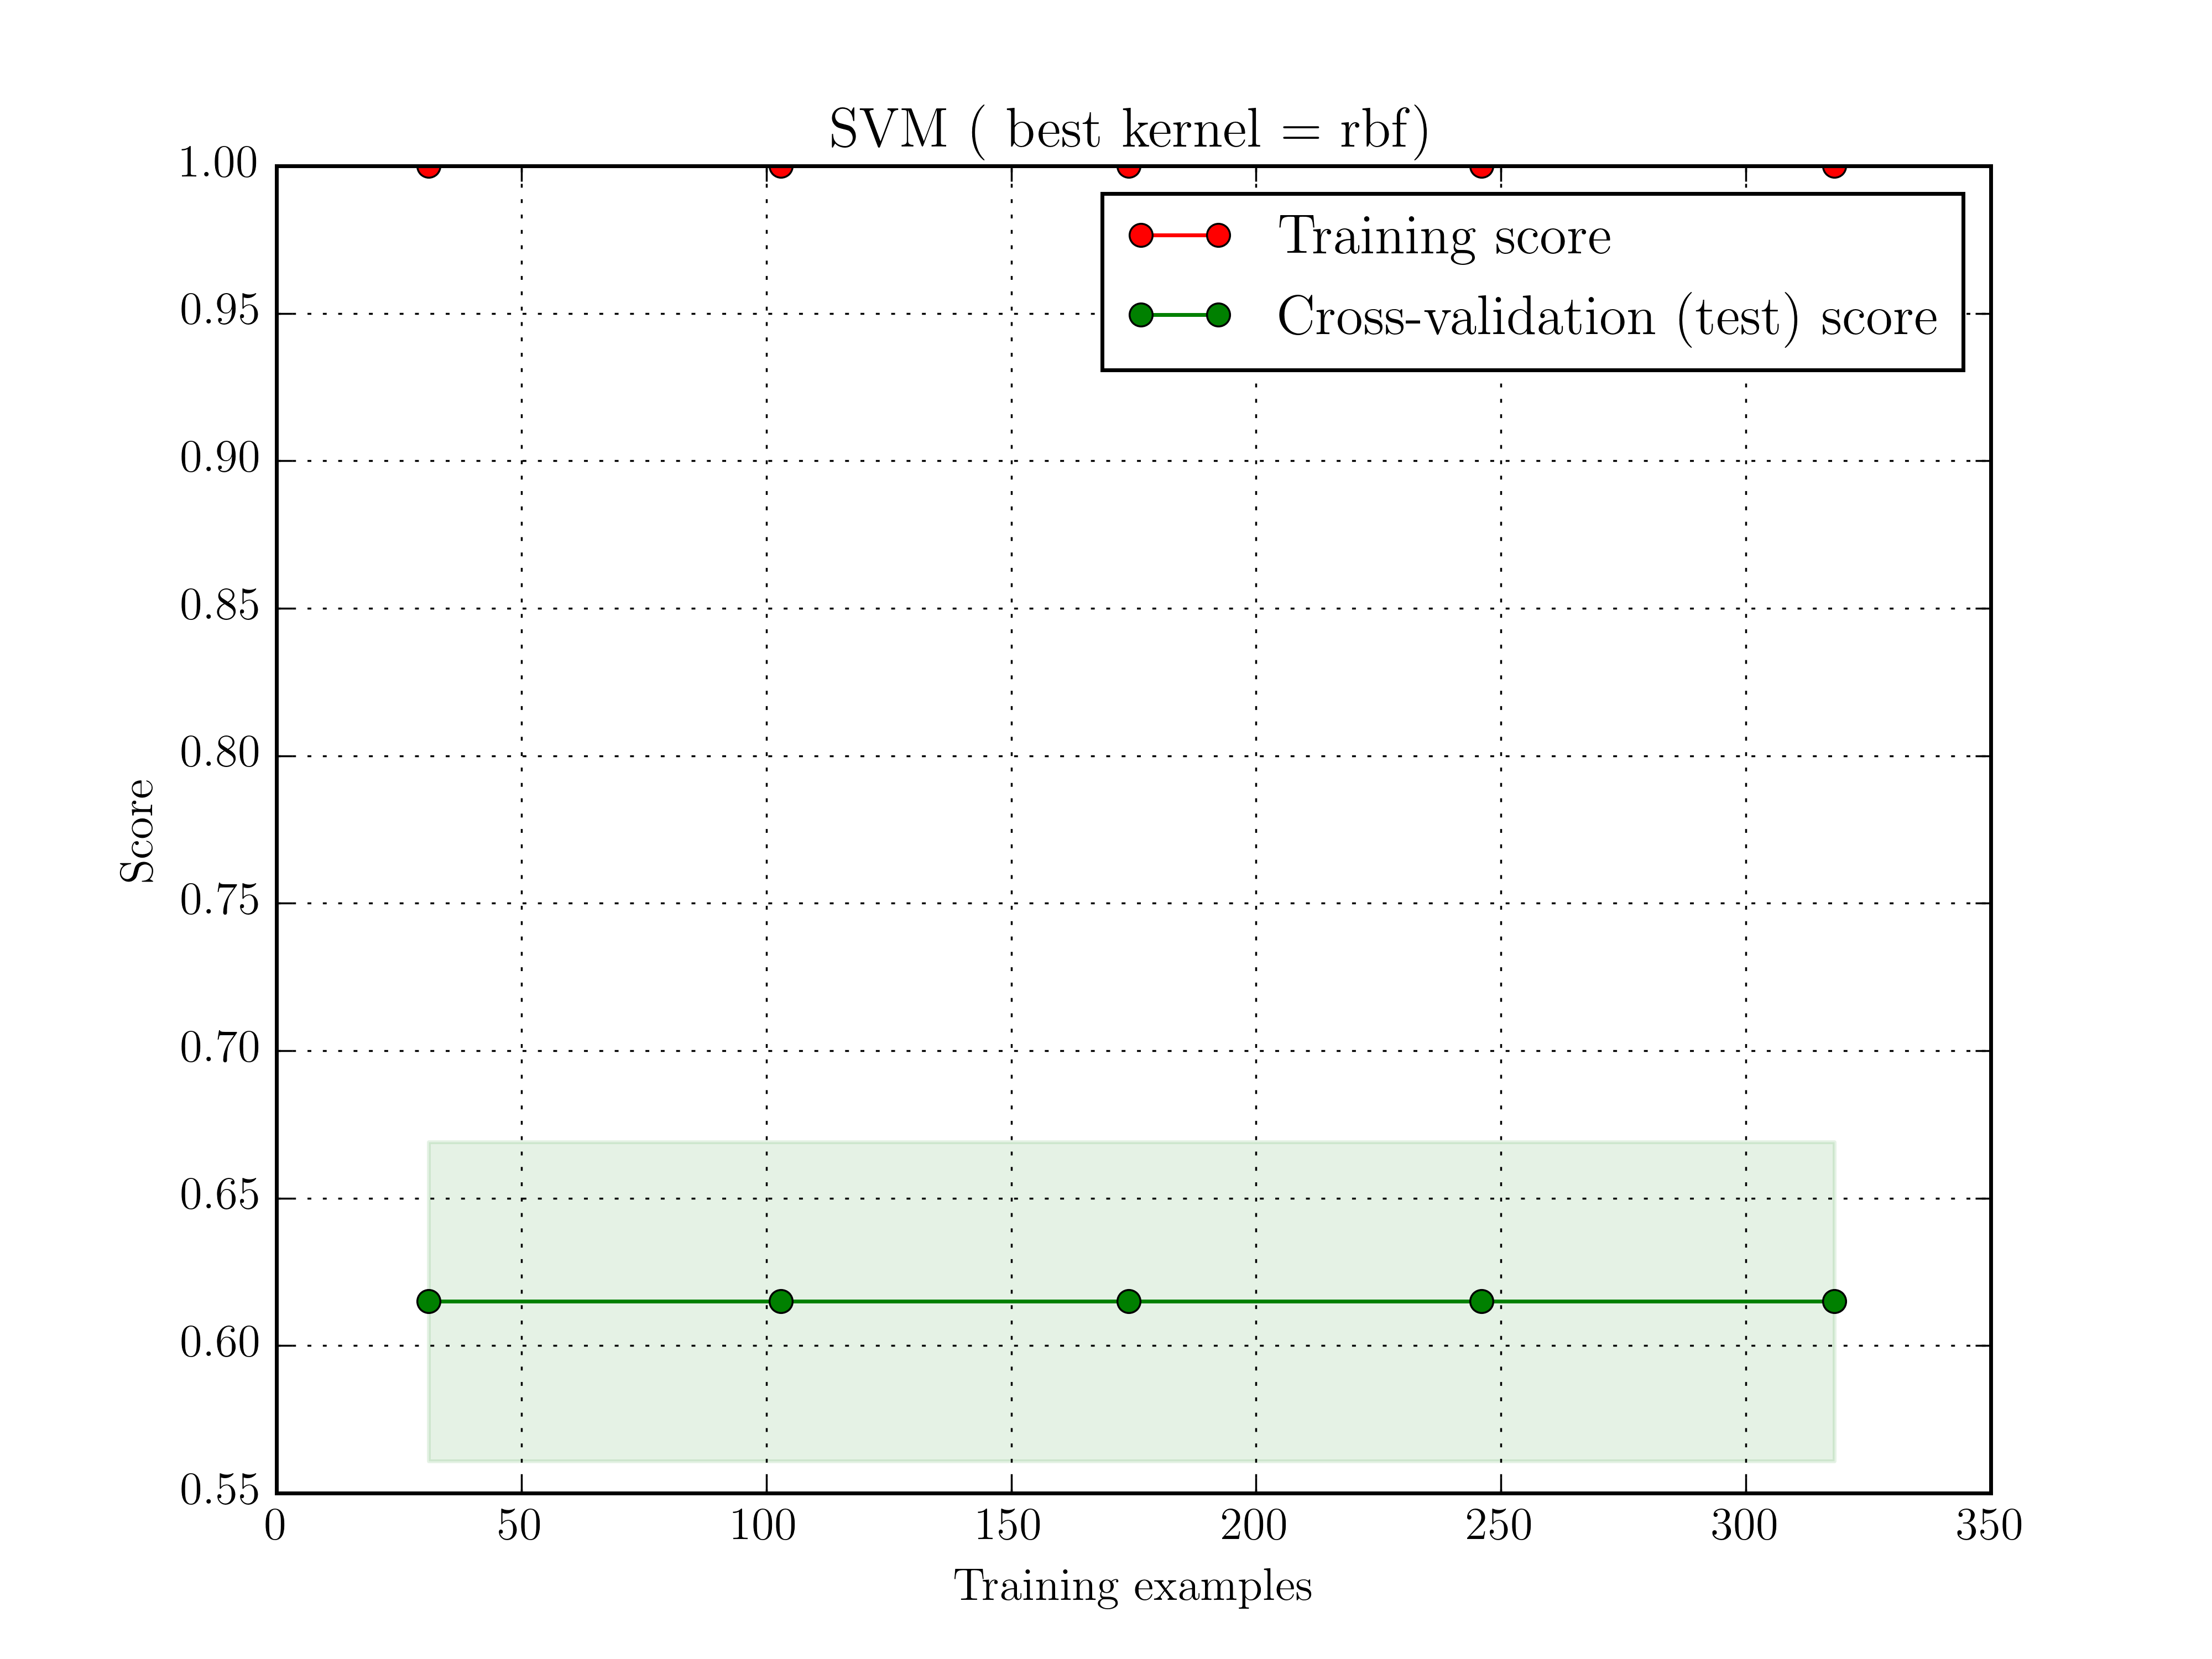
\includegraphics[width=.7\textwidth]{breast/svm.png}
    \caption{SVM on breast cancer data set. Runtime: 12 seconds}
\end{figure}

The following is a table for accuracy values for other kernels retrieved from the grid search algorithm.
The most accurate kernel (the one that is graphed) is shown in bold.
\begin{center}
    \begin{tabular}{l || l | l}
         kernel = & sigmoid & \textbf{radial basis function}\\
         \hline
         mean     & 0.608   & \textbf{0.612}\\
         std      & 0.024   & \textbf{0.068}
    \end{tabular}
\end{center}